\chapter{Data Analysis}

The PRex-II Experiment was conducted using the Jefferson Lab High-Resolution Spectrometer (JLab HRS). In this experiment, the kinematics of scattered electrons were measured using Vertical Drift Chambers (VDCs) positioned after the magnetic elements. It is crucial to transform these measurements back to the target coordinate system in order to obtain accurate results. This chapter delves into the details of JLab HRS calibration and the calculation of the squared four-momentum transfer.

\section{High-Resolution Spectrometer Coordinate System}


The Vertical Drift Chamber provides the HRS spatial resolution capability. Each of the two HRS spectrometers contains two Vertical Drift Chamber(VDC). Each chamber has 750 wires in two (U, V) planes, position resolution of 100 um per plane. Four VDC chamber layers of wires can provide partial spatial location $x$, $y$ together with particle angle $\theta$ and $\phi$. The kinematics, like scattered angle and scattered momentum, need to derive from the four direct measurable parameters(VDC $x$, $y$,$\theta$,$\phi$). The calibration procedure can be categorized into four steps:

\begin{itemize}
    \item VDC Drift time constant calibration
    \item VDC geometry constant calibration 
    \item spatial and angular calibration
    \item momentum calibration
\end{itemize}

Vertical Drift Chamber measures the spatial position by measuring the particle drift time. $t_0$ serves as the starting time of the VDC counter. Carefully calibrated $t_0$ is critical to the spatial and angular resolution of the VDC. To simplify the regression model and easily converge, the spatial, angular, and momentum parameters are calibrated from the focal plane. The VDC geometry constants are used to convert the direct measurements on the VDC plane to the focal plane. Before going into the detail of the calibration, here first introduce the coordination system used in the following contest. 

\subsection{coordinate system}


To simplify the calculation, couples of different coordinate systems are used. In this section, five coordinate systems and their directive relations are briefly introduced. A more detailed coordinate system of Jefferson Lab Hall A can be found in the ESPACE User Manual\cite{espace2002manual}.  

\subsubsection{Hall Coordinate System}
The center of the Hall Coordinate system is defined as the intersection of the electron beam and the vertical symmetry axis of the target system. $z$ is along the beam dump direction. $y$-axis is pointing vertically up against gravity.

[add HCS coordination plot]

\subsubsection{Target Coordinate System}

Each High-Resolution Spectrometer(HRS) has its own target coordinate system. Ideally, the center of the target coordinate system coincides with the center of the Hall A coordinate system. The distance from the hall A center to the midpoint of the center of the sieve slit hole is defined as $Z_0$ ($Z^{HRSE}_0 = 1.181 m$, $Z^{HRSH}_0 = 1.178 m$). The center of the target coordinate system is defined as $Z_0$ distance from the sieve slit(ref to chapter xx section xx) with $z$-axis perpendicular to the center of the sieve slit plane pointing to the beam direction. The $x$-axis is parallel to the sieve slit surface with $x$ pointing vertically down. The $\theta$ and $\phi$ angle is defined as $\frac{dx_{tg}}{Z_0}$ and $\frac{dy_{tg}}{Z_0}$ respectively.

[add TCS plot]


\subsubsection{Detector Coordinate System}

Each of the VDC chambers has 368 wires placed at $\pm 45 ^{\circ} u/v$ direction. The center of the detector coordinate system is defined as the intersection of wire 184 of the VDC1 U1 plane and the perpendicular projection of wire 184 in the VDC1 V1 plane onto the VDC1 U1 plane. $x$-axis is along the long edge of the VDC plane, while y is along the short edge of the VDC plane and $z$ is perpendicular to the VDC plane and pointing upwards. 

Let's take $p_{vdc,n}$ (where ${n=1-4}$)to be the cross position of a particle with each VDC plane. The vertex can be calculated with the following equation. 

\begin{equation}
    \tan \eta_{1} = \frac{p_{vdc,3} - p_{vdc, 1}}{d1}    
\end{equation}
\begin{equation}
    \tan \eta_{2} = \frac{p_{vdc,4} - p_{vdc, 2}}{d1}    
\end{equation}

For ideal experimental configurations, we take the following assumptions:
\begin{enumerate}
    \item All the VDC wires are positioned on a 2D VDC plane
    \item All the VDC wires are oriented in $45\circ$ angle
    \item there is no distortion with the VDC wires
    \item all the VDC frames a perfect parallel to each other 
    \item the center of each VDC plane is known with no error
\end{enumerate}

Given the above assumption, The trajectory position and vertex angles in the detector plane coordinate system can be derived with the following equation 

\begin{equation}
    \theta_{det} = \frac{\tan{\eta_1} + \tan{\eta_2}}{\sqrt{2}}
\end{equation}
    
\begin{equation}
    \phi_{det} =  \frac{-\tan{\eta_1} + \tan{\eta_2}}{\sqrt{2}}
\end{equation}

\begin{equation}
    x_{det} = \frac{p_{vdc,1} + (p_{vdc,2} - d_1\tan{\eta_2})}{\sqrt{2}}
\end{equation}

\begin{equation}
    y_{det} = \frac{-p_{vdc,1} + (p_{vdc,2} - d_1\tan{\eta_2})}{\sqrt{2}}
\end{equation}

Even though the VDC could not be ideal, the distortions would be very small and through HRS Optics, those un-idea errors could be corrected. 

In Hall A analyzer, the VDC result will be given in the detector plane coordinate system.

[add vdc, DCS plot]

\subsubsection{Transport Rotation Coordinate System at the focal plane}
The transport coordinate system at the focal plane is defined as rotating the detector coordinate system by $45^{\circ}$ along the y-axis. Ideally the z-axis along the central beam ray. 

Given the particle position at the detector coordinate system, the transport rotation coordinate system can be derived as:

\begin{equation}
    \theta_{tra}  = \frac{\theta_{det} + \tan{\rho_0}}{1 - \theta_{det}\tan{\rho_0}} 
\end{equation}

\begin{equation}
    \phi_{tra} = \frac{\phi_{det}}{\cos{\rho_0} - \theta_{det}\sin{\rho_0}}
\end{equation}

\begin{equation}
    x_{tra} = x_{det}\cos{\rho_0}(1 + \theta_{det}\sin{\rho_0})
\end{equation}

\begin{equation}
    y_{tra} = y_{det} + \sin{\rho_0}\phi_{tra}x_{det}
\end{equation}


[add the plot of the transport coordinate system plot]


\subsubsection{Focal plane Coordinate System}

The focal plane coordinate system used for HRS analysis is a rotated coordinate system, obtained by rotating the Detector Coordinate System (DCS) around its y-axis by an angle. This angle is determined by the angle between the local central ray and the z-axis of the DCS, and as a result, the z-axis of the Focal Plane Coordinate System (FCS) rotates as a function of the relative momentum p. Because of the focusing of HRS magnet system,  particle from different scattering angles with same momentum will be focused at the focal plane. therefore, the relative momentum to the central momentum of the spectrometer which defined as 
\begin{equation}
    \delta = \frac{p-p_0}{p_0}
\end{equation}

this factor approximately only depends on $x_{tra}$ and $p_0$.

To ensure easy convergence, the HRS Optics Tensor is calibrated with respect to the angles $\theta$ and $\phi$, the vertical position $y$, and the relative momentum $dp$ on the Focal Plane Coordinate System.

\begin{equation}
    x_fp = x_{tra}    \label{eq:cpt3_fps_1}
\end{equation}

\begin{equation}
    y_{fp} = y_{tra} - \sum y_{i000}x^i_{fp}  
\end{equation}

\begin{equation}
\theta_{fp} = \frac{\theta_{det} + \tan\rho}{1 - \theta_{det}\tan\rho}
\end{equation}


\begin{equation}
    \phi_{fp} = \frac{\phi_{det} - \sum p_{i000}x^i_{fp}}{cos \rho - \theta_{det} sin\rho}
\end{equation}

here  in the equation:

\begin{equation}
    \tan\rho  = \sum t_{i000}x^i_{fp} \label{eq:cpt3_fps_5}
\end{equation}


the code used for calibration of the focal plane constant can be found on this GitHub repository: \href{https://github.com/Jiansiyu/GeneralScripts/blob/master/vdcConstantOpt}{GitHub Repository Link}


[need to add the Focal plane coordination system plot]


\section{Vertical Drift Chamber $T_0$ calibration}

Each High-Resolution Spectrometer (HRS) is outfitted with a set of four Vertical Drift Chambers (VDCs) arranged in the UV direction. These VDCs are filled with a mixture of Argon (Ar) and flammable ethane, which is bubbled through alcohol. The gas mixture is managed and supplied by the Hall A Gas System. Every wire within the VDCs is connected to a 3.5 kV high-voltage source.

[Explain the VDC electronics and emphasize the importance of an accurate $T_0$]

When a charged particle traverses the VDC chamber, it ionizes the gas atoms, generating a trail of ionized electrons along its trajectory. The ionized electrons drift along the electric field lines due to the high voltage applied between the high voltage plane and the signal wires. This ionization process produces a pulse on the signal wires. Each VDC chamber contains 368 wires, all connected to a pre-amplifier. The amplified pulse signal is subsequently passed through a discriminator and utilized to trigger the Time-Digital Converter (TDC). The TDC is stopped by the overall event trigger from Hall A.

As the particle passes through the chamber, it typically activates a cluster comprising 4-6 wires. The intersection between the particle's trajectory and the VDC plane can be determined by measuring the drift distance between each wire, as illustrated in Fig \ref{fig:vdc_wire_ionization_cluster}. The drift distance is calculated using the drift time obtained from the Time-Digital Converter. An accurate start time is crucial for determining the precise drift distance and, consequently, the exact position on the VDC. If the threshold is set too high or too low, the VDC drift distance will be biased. An example of an improper $T_0$ setting is depicted in the plot, where numerous 'wire shadows' can be seen. These shadows are the result of measurement biases. 

Before the HRS Calibration, the VDC $T_0$ need to calibrate to get a reliable VDC data. 
\begin{figure}[!htbp]
    \centering
    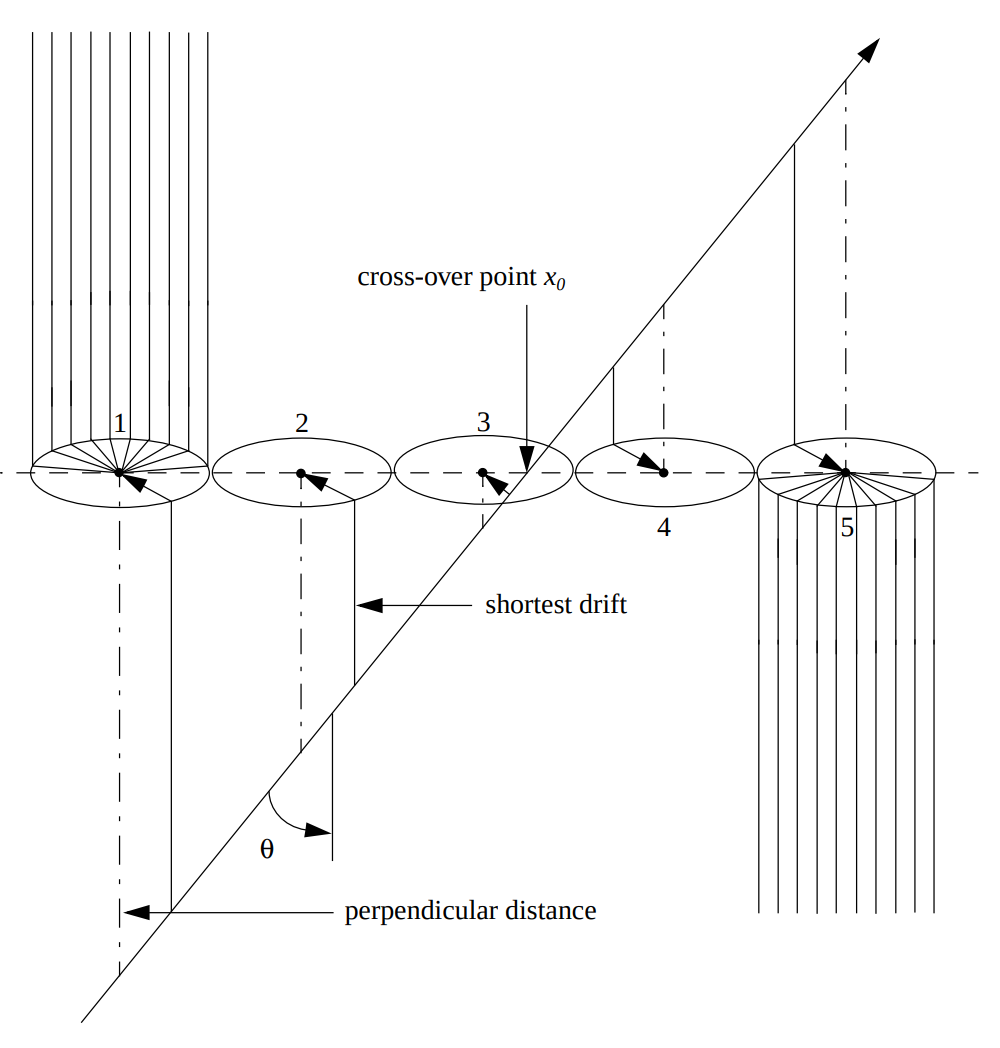
\includegraphics[scale = 0.25]{images/chap4/vdc_wire_ionize.png}
    \caption{Vertical Drift Chamber Ionization (need to redraw)}
    \label{fig:vdc_wire_ionization_cluster}
\end{figure}

\begin{figure}[!htbp]
    \centering
    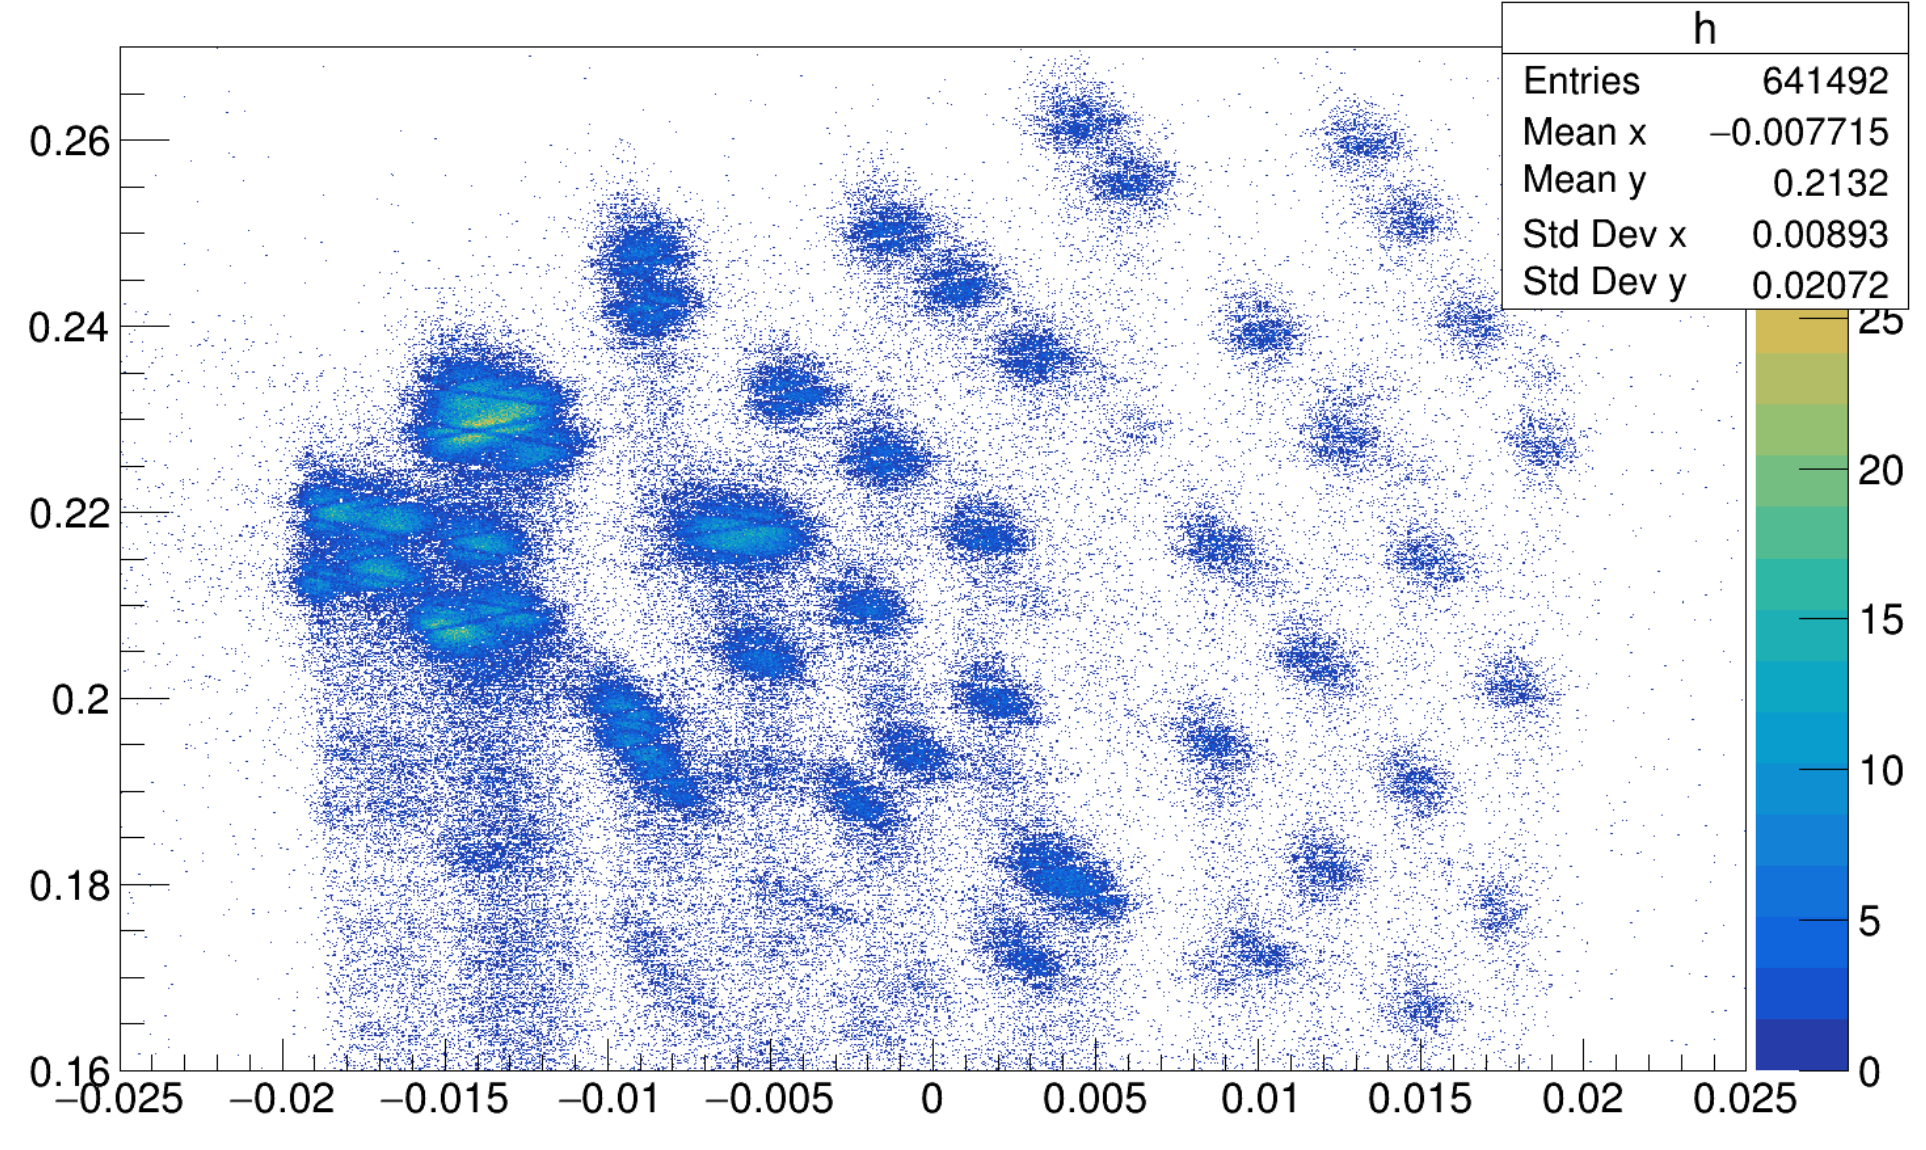
\includegraphics[width=\textwidth]{images/chap4/vdc_t0_before_correction.png}
    \caption{vdc $x$ vs $y$ on vdc detector plane before $T_0$ correction}
    \label{fig:vdc_t0_before_correction}
\end{figure}
\subsection{correction the initial drift time $T_0$}

The spatial position of the VDC is determined by measuring the drift time. A typical data frame of a single VDC chamber signal channel is presented below. It features a peak followed by a flat tail, which is caused by the drift time of the ionized ions. In practice, the start time $T_0$ is chosen as the $1.4\sigma$ time of the ionized electron rising peak, and the VDC wires are grouped by 16 wires.

\begin{figure}[!htbp]
\centering
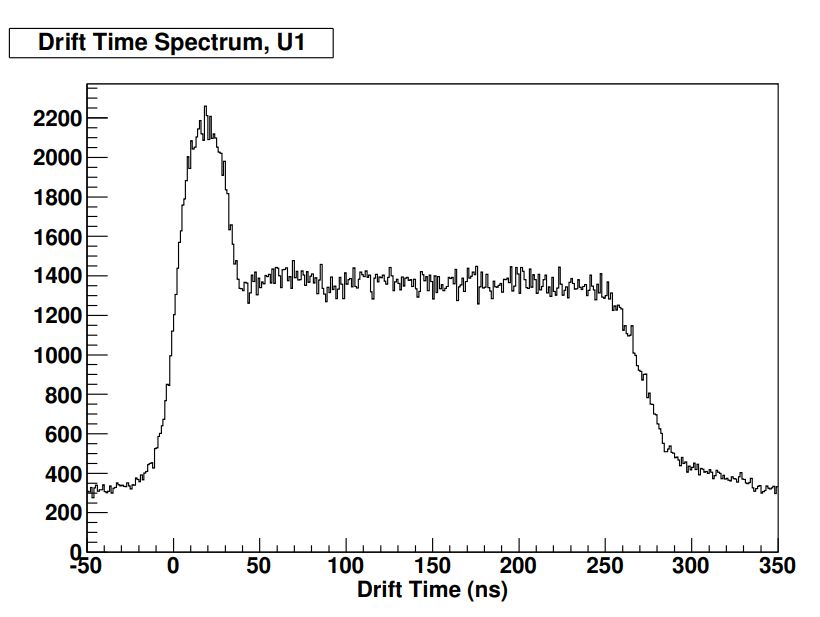
\includegraphics[scale = 0.25]{images/chap4/vdc_signals.png}
\caption{VDC Drift Time Spectrum}
\label{fig:vdc_dift_time_spectrum}
\end{figure}

To calibrate the TDC for the entire VDC range, data from white spectrum runs covering the full focal plane range with high statistics are required. In the experiment, a carbon target without a sieve slide was used.

The following is a calibration procedure for the TDC $T_0$: 
\begin{enumerate}
\item Fit the falling tail of the spectrum.
\item Identify the point 1.4 $\sigma$ before the peak time.
\item Calculate the $1.4\sigma$ time for all events, and use the average as the final $T_0$ for the given channel.
\end{enumerate}

Figure \ref{fig:vdc_t0_after_correction} shows the sieve slide pattern on the focal coordinate system. After correcting the $T_0$, the 'shadow pattern' is corrected.

\begin{figure}
\centering
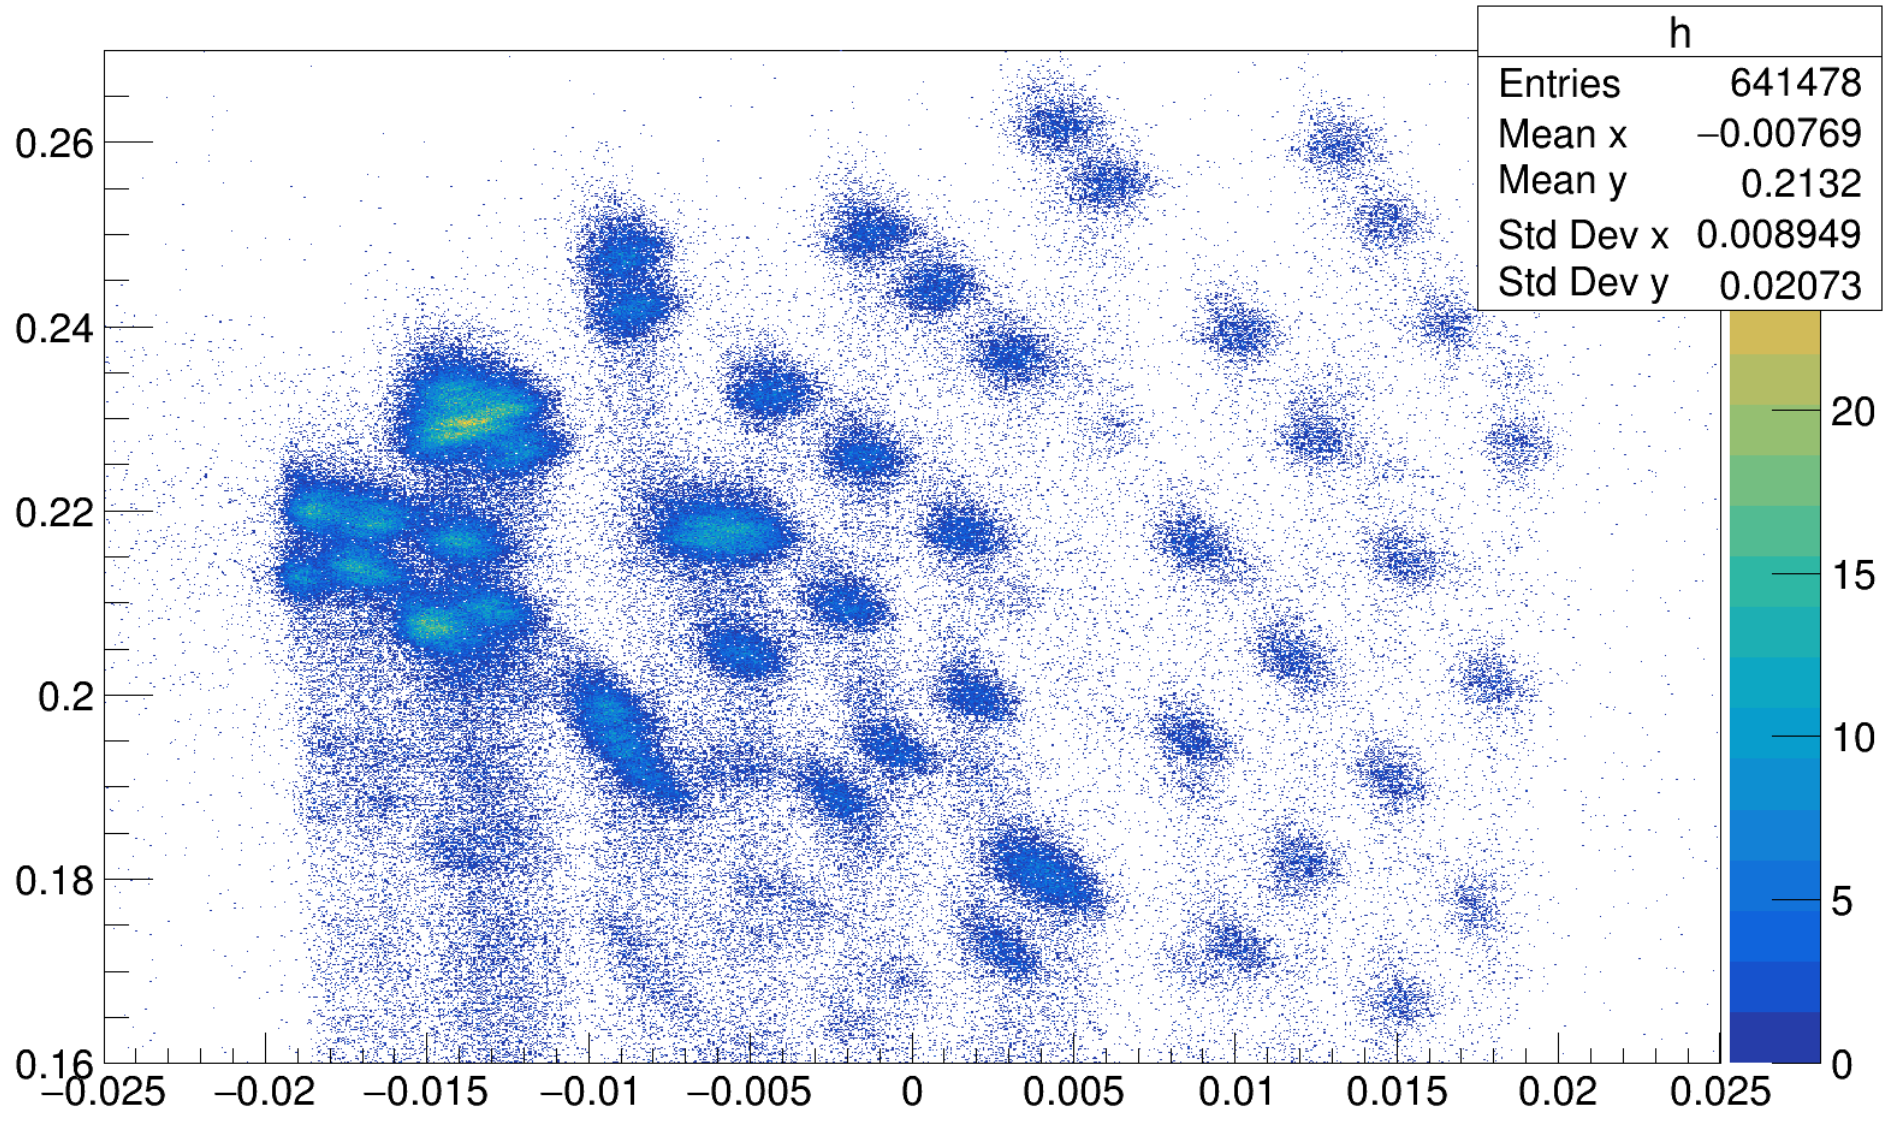
\includegraphics[width=\textwidth]{images/chap4/vdc_t0_after_correction.png}
\caption{VDC $x$ vs $y$ on the VDC detector plane after $T_0$ correction}
\label{fig:vdc_t0_after_correction}
\end{figure}


The calibration code can be found in this \href{https://github.com/Jiansiyu/GeneralScripts/tree/master/VDC_T0_Cali}{GitHub repository}  



\section{focal plane constant calibration}

The HRS Spectrometer Focal Plane Coordinate System is a rotated system, with the Z-axis being the projection of the local central ray on the x-z plane. The origin of this coordinate system is shared with the detector coordinate system. To correct the coordinate system, we use a criterion based on the ideal case of the central beam passing through the central sieve hole, where the beam position is (0,0). Specifically, we look at the equation of the focal plane coordinate system, where a parameter is used to project the coordinate system. To achieve high accuracy, each parameter is optimized to the 3rd order.

In the Hall A analyzer, the correction constant can be found in the first three rows of the x.vdc.matrixelem variable:

\begin{center}
    \begin{tabular}{|c c c c | c c c c|} \hline
        t & 0 & 0 & 0 & -1.001135e+00 & -3.313373e-01 & -4.290819e-02 & 4.470852e-03 \\
        y & 0 & 0 & 0 & -8.060915e-03 & 1.071977e-03 & 9.019102e-04 & -3.239615e-04 \\
        p & 0 & 0 & 0 & -2.861912e-03 & -2.469069e-03 & 8.427172e-03 & 2.274635e-03 \\ \hline
    \end{tabular}
    \caption{focal plane correction constant}
\end{center}

Here, the first column indicates the parameter name, followed by the orders of $\theta$, $\phi$, and $dp$ (all 0s in this case), and the constant factors of $x^0$, $x^1$, $x^2$, $x^3$.

According to the focal plane coordinate system definition, for the central beam passing through the central sieve hole, we have $\theta_{focal}=0$, $\phi_{focal}=0$, and $y_{focal}=0$.

To optimize the correction constant, we follow these steps:

\begin{enumerate}
    \item Gather as many runs as possible at any central P runs.
    \item Select the events that pass through the central sieve hole.
    \item Calculate the detector plane parameters for all the events.
    \item Define the loss function as the square residual of the focal plane calculated using the detector coordinate variables (given by equations \ref{eq:cpt3_fps_1} to \ref{eq:cpt3_fps_5}) and the theoretical value of 0.
    \item Optimize the loss using a linear regression model, and obtain the constants $t_{i000}$, $y_{i000}$, and $p_{i000}$.
\end{enumerate}


\begin{figure}
    \centering
    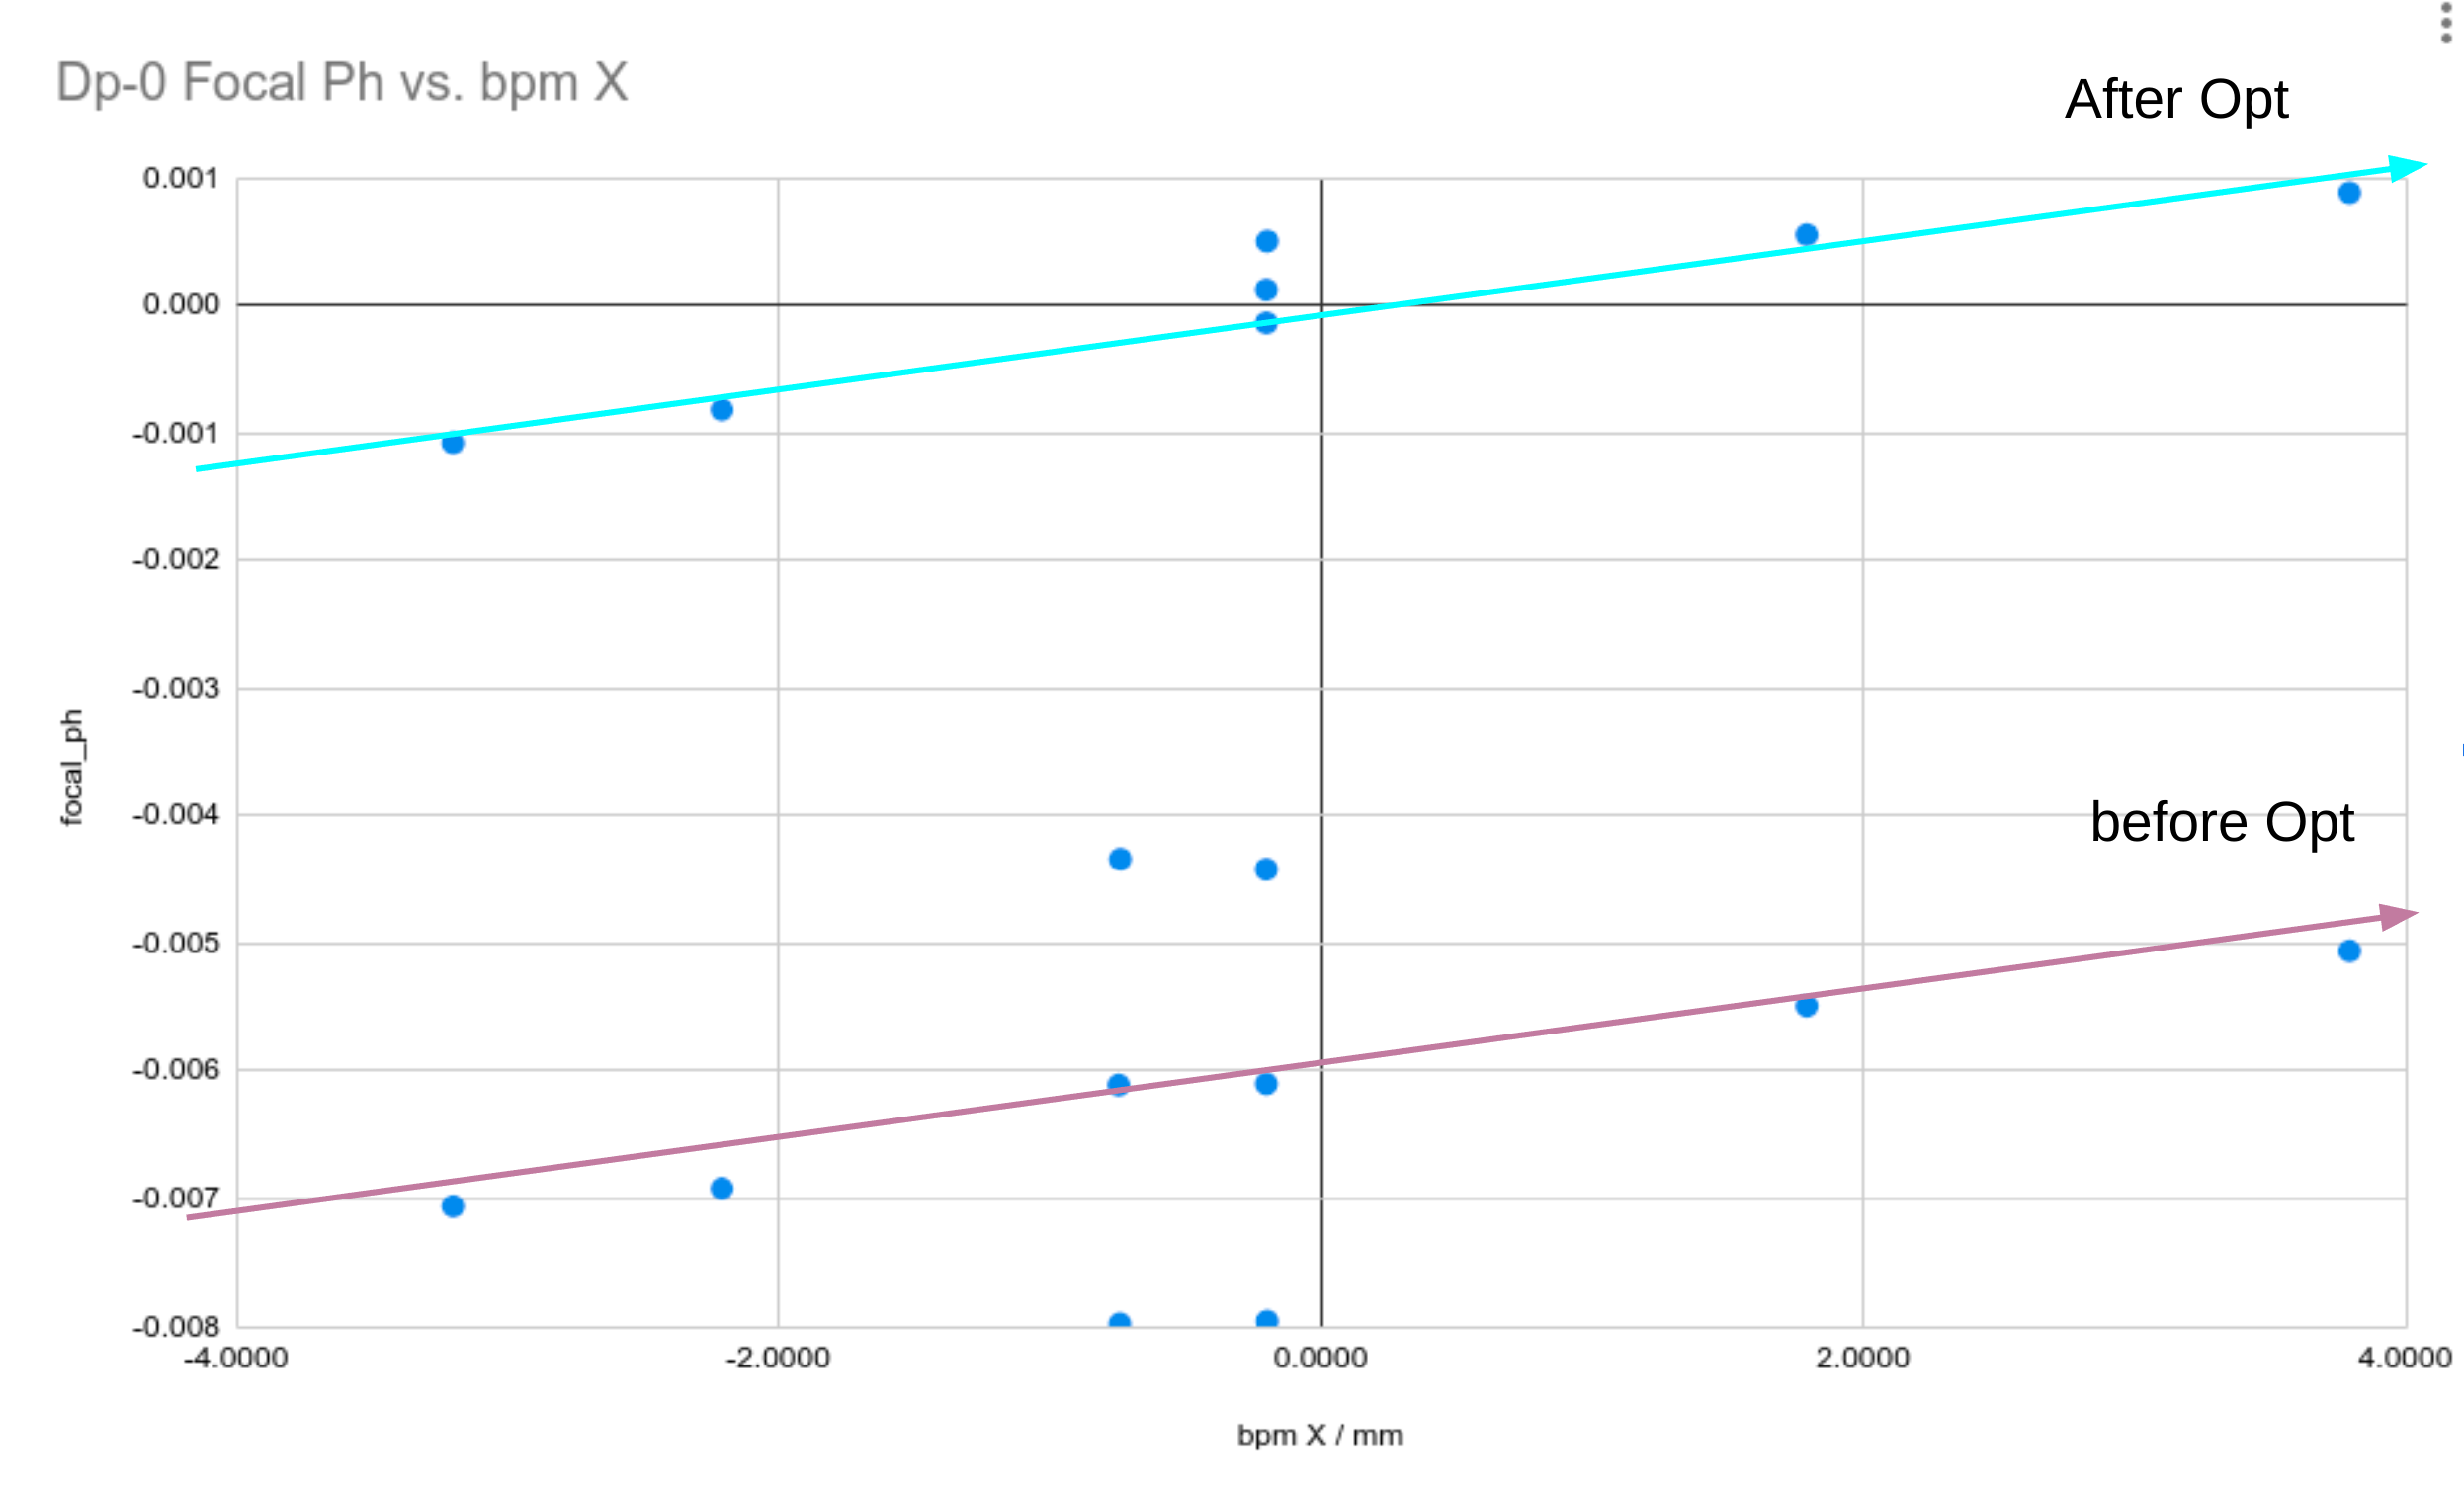
\includegraphics[width =\textwidth]{images/chap4/vdcconstant_focal_bpmx.png}
    \caption{$\phi_{focal}$ vs. $x_{bpm}$ before and after focal plane constant correction [to be replaced]}
    \label{fig:focal_ph_bpm_x_constant_correction_plt}
\end{figure}


\begin{figure}
    \centering
    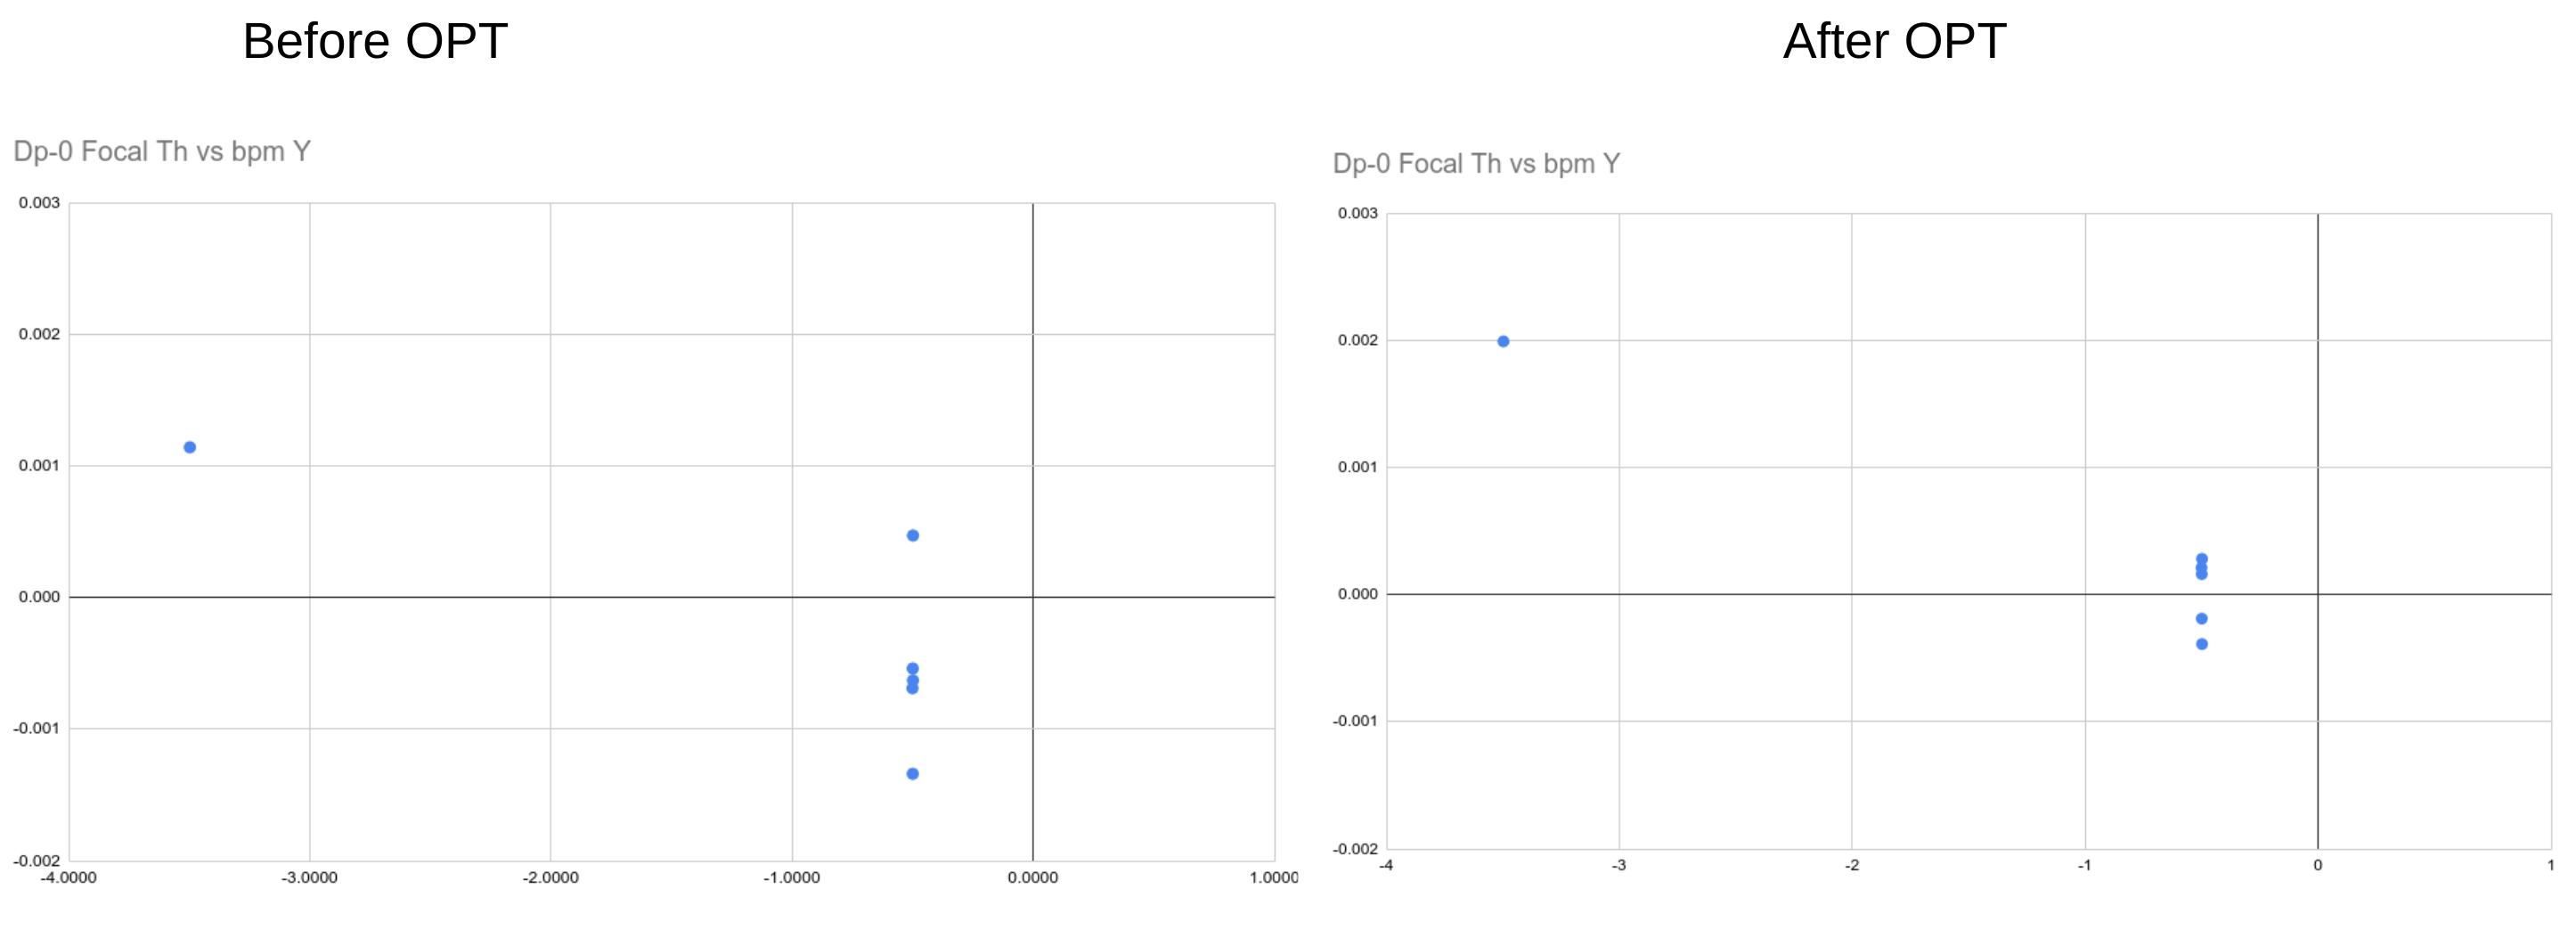
\includegraphics[width =\textwidth]{images/chap4/vdcconstant_focal_th_bpmy.png}
    \caption{$\theta_{focal}$ vs. $y_{bpm}$ before and after focal plane constant correction [to be replaced]}
    \label{fig:my_label}
\end{figure}

\begin{figure}
    \centering
    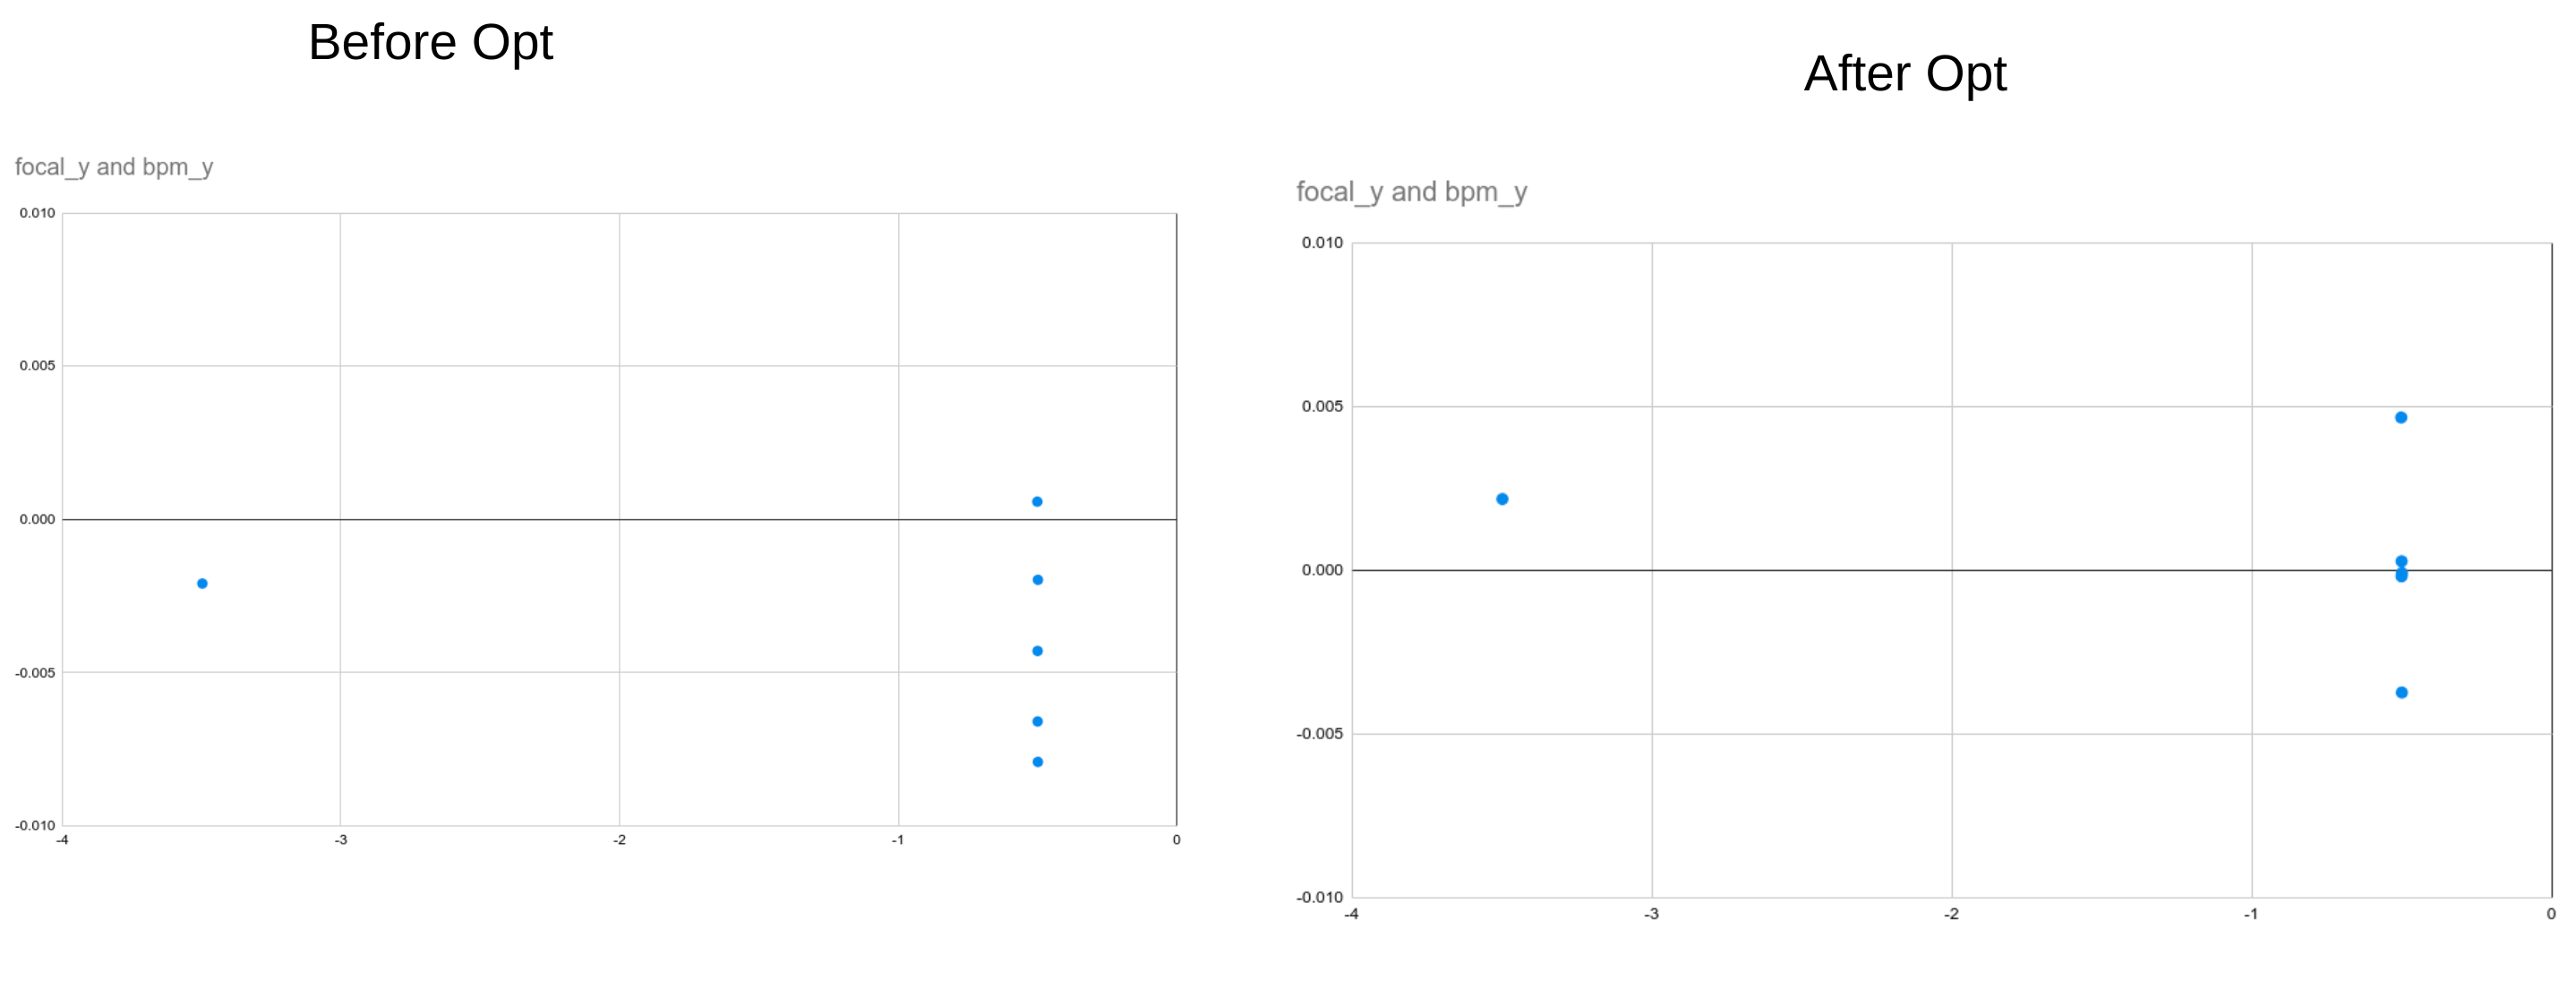
\includegraphics[width =\textwidth]{images/chap4/vdcconstant_focaly_bpmy.png}
    \caption{$y_{focal}$ vs. $x_{bpm}$ before and after focal plane constant correction [to be replaced]}
    \label{fig:my_label}
\end{figure}

From the plot we could see, after the optimization, with the new constant $t_{i000}$,$y_{i000}$,$p_{i000}$, the central sieve $\theta_{focal}$,$\phi_{focal}$,$y_{focal}$ are set to $(0,0,0)$.


\section{High-Resolution Spectrometer Calibration}

In the preceding section, we introduced the calibration process used to map the detector coordinate system onto the focal plane coordinate system. In this section, we will delve into HRS Optics, specifically focusing on the transformation from the focal plane coordinate system to the target coordinate system.

\subsection{Approach}

With the previous introduction, the direct measurement the position on the 4 vertical drift chambers $p_{vdc,i}$ together with the displacement of the chambers $d$ are converted to the focal plane coordinate system, $x_{fp}$,$y_{fp}$,$\theta_{fp}$,$\phi_{fp}$. Those observables are used to calculate $\theta_{tg}$,$\phi_{tg}$,$y_{tg}$, and $\delta_{tg}$ on the target which we used for further physics analysis. 

The conversion from the focal plane coordinate system to the target coordinate system is with the transport tensors. In first-order approximation, the relation between the two coordinate systems can be written as:

\begin{equation}
\begin{bmatrix}
\delta_{tg} \\
\theta_{tg} \\
y_{tg} \\
\phi_{tg}
\end{bmatrix} = \begin{bmatrix}
    <x_{fp}|x_{fp}> & <x_{fp}|\theta_{fp}> & 0 & 0 \\
    <\theta_{fp}|x_{fp}> & <\theta_{fp}|\theta_{fp}> & 0 & 0 \\
    0 & 0 & <y_{fp}|y_{fp}> & <y_{fp}|\phi_{fp}>  \\
    0 & 0 & <\phi_{fp}|y_{fp}> & <\phi_{fp}|\phi_{fp}>  
\end{bmatrix} * \begin{bmatrix}
    x_{fp} \\
    \theta_{fp} \\
    y_{fp} \\
    \phi_{fp}
\end{bmatrix}
\end{equation}

Because of the mid-plane symmetry of the spectrometer, 8 of the reverse corner element are $0$.'

% explain why it is to $$x^n$$ order? what is the physics meaning of 

In practice, the expansion of the focal plane coordinates is performed up to the fifth order and use the polynomial production of the four observables as features in modeling the spectrum. 

\begin{equation}
    y_{tg} = \sum_{jkl}Y_{jkl}\theta^j_{fp}y^k_{fp}\phi^l_{fp}
\end{equation}


\begin{equation}
    \theta_{tg} = \sum_{jkl}T_{jkl}\theta^j_{fp}y^k_{fp}\phi^l_{fp}
\end{equation}


\begin{equation}
    \phi_{tg} = \sum_{jkl}P_{jkl}\theta^j_{fp}y^k_{fp}\phi^l_{fp}
\end{equation}


\begin{equation}
    \delta_{tg} = \sum_{jkl}D_{jkl}\theta^j_{fp}y^k_{fp}\phi^l_{fp}
\end{equation}

Where in the above equations, tensors $Y_{jkl}$, $T_{jkl}$, $P_{jkl}$, $D_{jkl}$ are are polynomial of $x_fp$ for example, $Y_{ijk}$ can be write as:

\begin{equation}
    Y_{jkl} = \sum^m_{i=1}C_i^{Y_{jkl}}x^i_{fp}
\end{equation}

In the equation, $C^i_{jkl}$ is the $x^i$ correction constant for $Y_{jkl}$. The final equation can be written as:

\begin{equation}
    y_{tg} = \sum_{jkl} (\sum^m_{i=1}C_i^{Y_{jkl}}x^i_{fp}) \theta^j_{fp}y^k_{fp}\phi^l_{fp}
\end{equation}


\begin{equation}
    \theta_{tg} = \sum_{jkl}(\sum^m_{i=1}C_i^{T_{jkl}}x^i_{fp})\theta^j_{fp}y^k_{fp}\phi^l_{fp}
\end{equation}


\begin{equation}
    \phi_{tg} = \sum_{jkl}(\sum^m_{i=1}P_i^{Y_{jkl}}x^i_{fp})\theta^j_{fp}y^k_{fp}\phi^l_{fp}
\end{equation}


\begin{equation}
    \delta_{tg} = \sum_{jkl}(\sum^m_{i=1}D_i^{Y_{jkl}}x^i_{fp})\theta^j_{fp}y^k_{fp}\phi^l_{fp}
\end{equation}

Here is an example of Y in the vertical drift chamber database:

\begin{center}
    % \captionof{focal plane correction constant}
    \begin{tabular}{c c c c c c c }
        D& 0& 0& 0&  8.851691E-04& 7.570314E-02& 1.116963E-02\\
        D& 0& 0& 1&  4.667677E-02& 9.485094E-02&
    \end{tabular}    
\end{center}

In the first row, $D$ indicates this is the tensor for the $\delta_{tg}$, the following three integers is corresponding to the power of $\theta$,$y$,$\phi$, which is $jkl$ in the equation. The following float number is the $i=1$ constant, $i=2$ constant and etc. 


To achieve high optics accuracy, each element is optimized up to the fifth order. Because of the overfitting issue if there are too many features present in the model, in the optimization practice, not all the orders are kept for each tensor. In the training process, each feature is carefully tested to make sure it will not cause serious overfitting and get the best test result on the holdout dataset. 

[add how to select the features that most suitable for the model??]

\subsection{Ground Truth data set}

In order to construct a precise regression model for the HRS spectrometer, a highly accurate ground truth dataset is essential. This ground truth is derived from a meticulously crafted CNC-made sieve plate. It is a stainless steel plane with holes in the grid. Every hole is manufactured with a high accurate cnc machine. With the given position of each sieve hole, we can calculate the theoretical value for the scattering angle as well as the momentum for each sieve hole. Those sieve holes provide us with an accurate calibration point for the HRS. 

The sieve plate is strategically positioned in front of the septum magnet, with its location carefully surveyed to ensure a positional accuracy of up to 100 micrometers. As electrons scatter from the target, only those that pass through the holes on the sieve plate are allowed to enter the spectrometer and ultimately reach the vertical drift chamber. All other electrons are effectively blocked by the sieve plate.

Upon reaching the vertical drift chamber, particles that have passed through the same hole on the sieve plate will form a distinct cluster. By categorizing events based on these clusters and considering the relative positions of the clusters on the sieve plate, it is possible to determine which holes the particles have originated from. With this information, the ground truth values can be calculated for each sieve hole.

In the following sections, we will delve into the details of calculating the ground truth values used to calibrate the HRS spectrometer, ensuring the highest level of accuracy and precision in the model.

\subsubsection{apparatus [need to rewrite]}

\begin{figure}
    \centering
    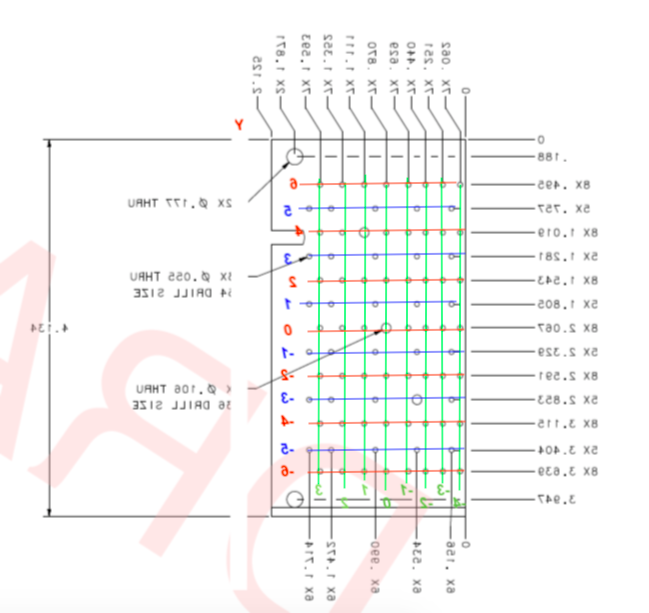
\includegraphics[width =\textwidth]{images/chap4/sieve_cnc_draw.png}
    \caption{PRex-II sieve slit used for Optics Calibration, three big holes are used for identifying the orientation of the reconstructed data}
    \label{fig:sieve_cnc_draw}
\end{figure}


\begin{figure}
    \centering
    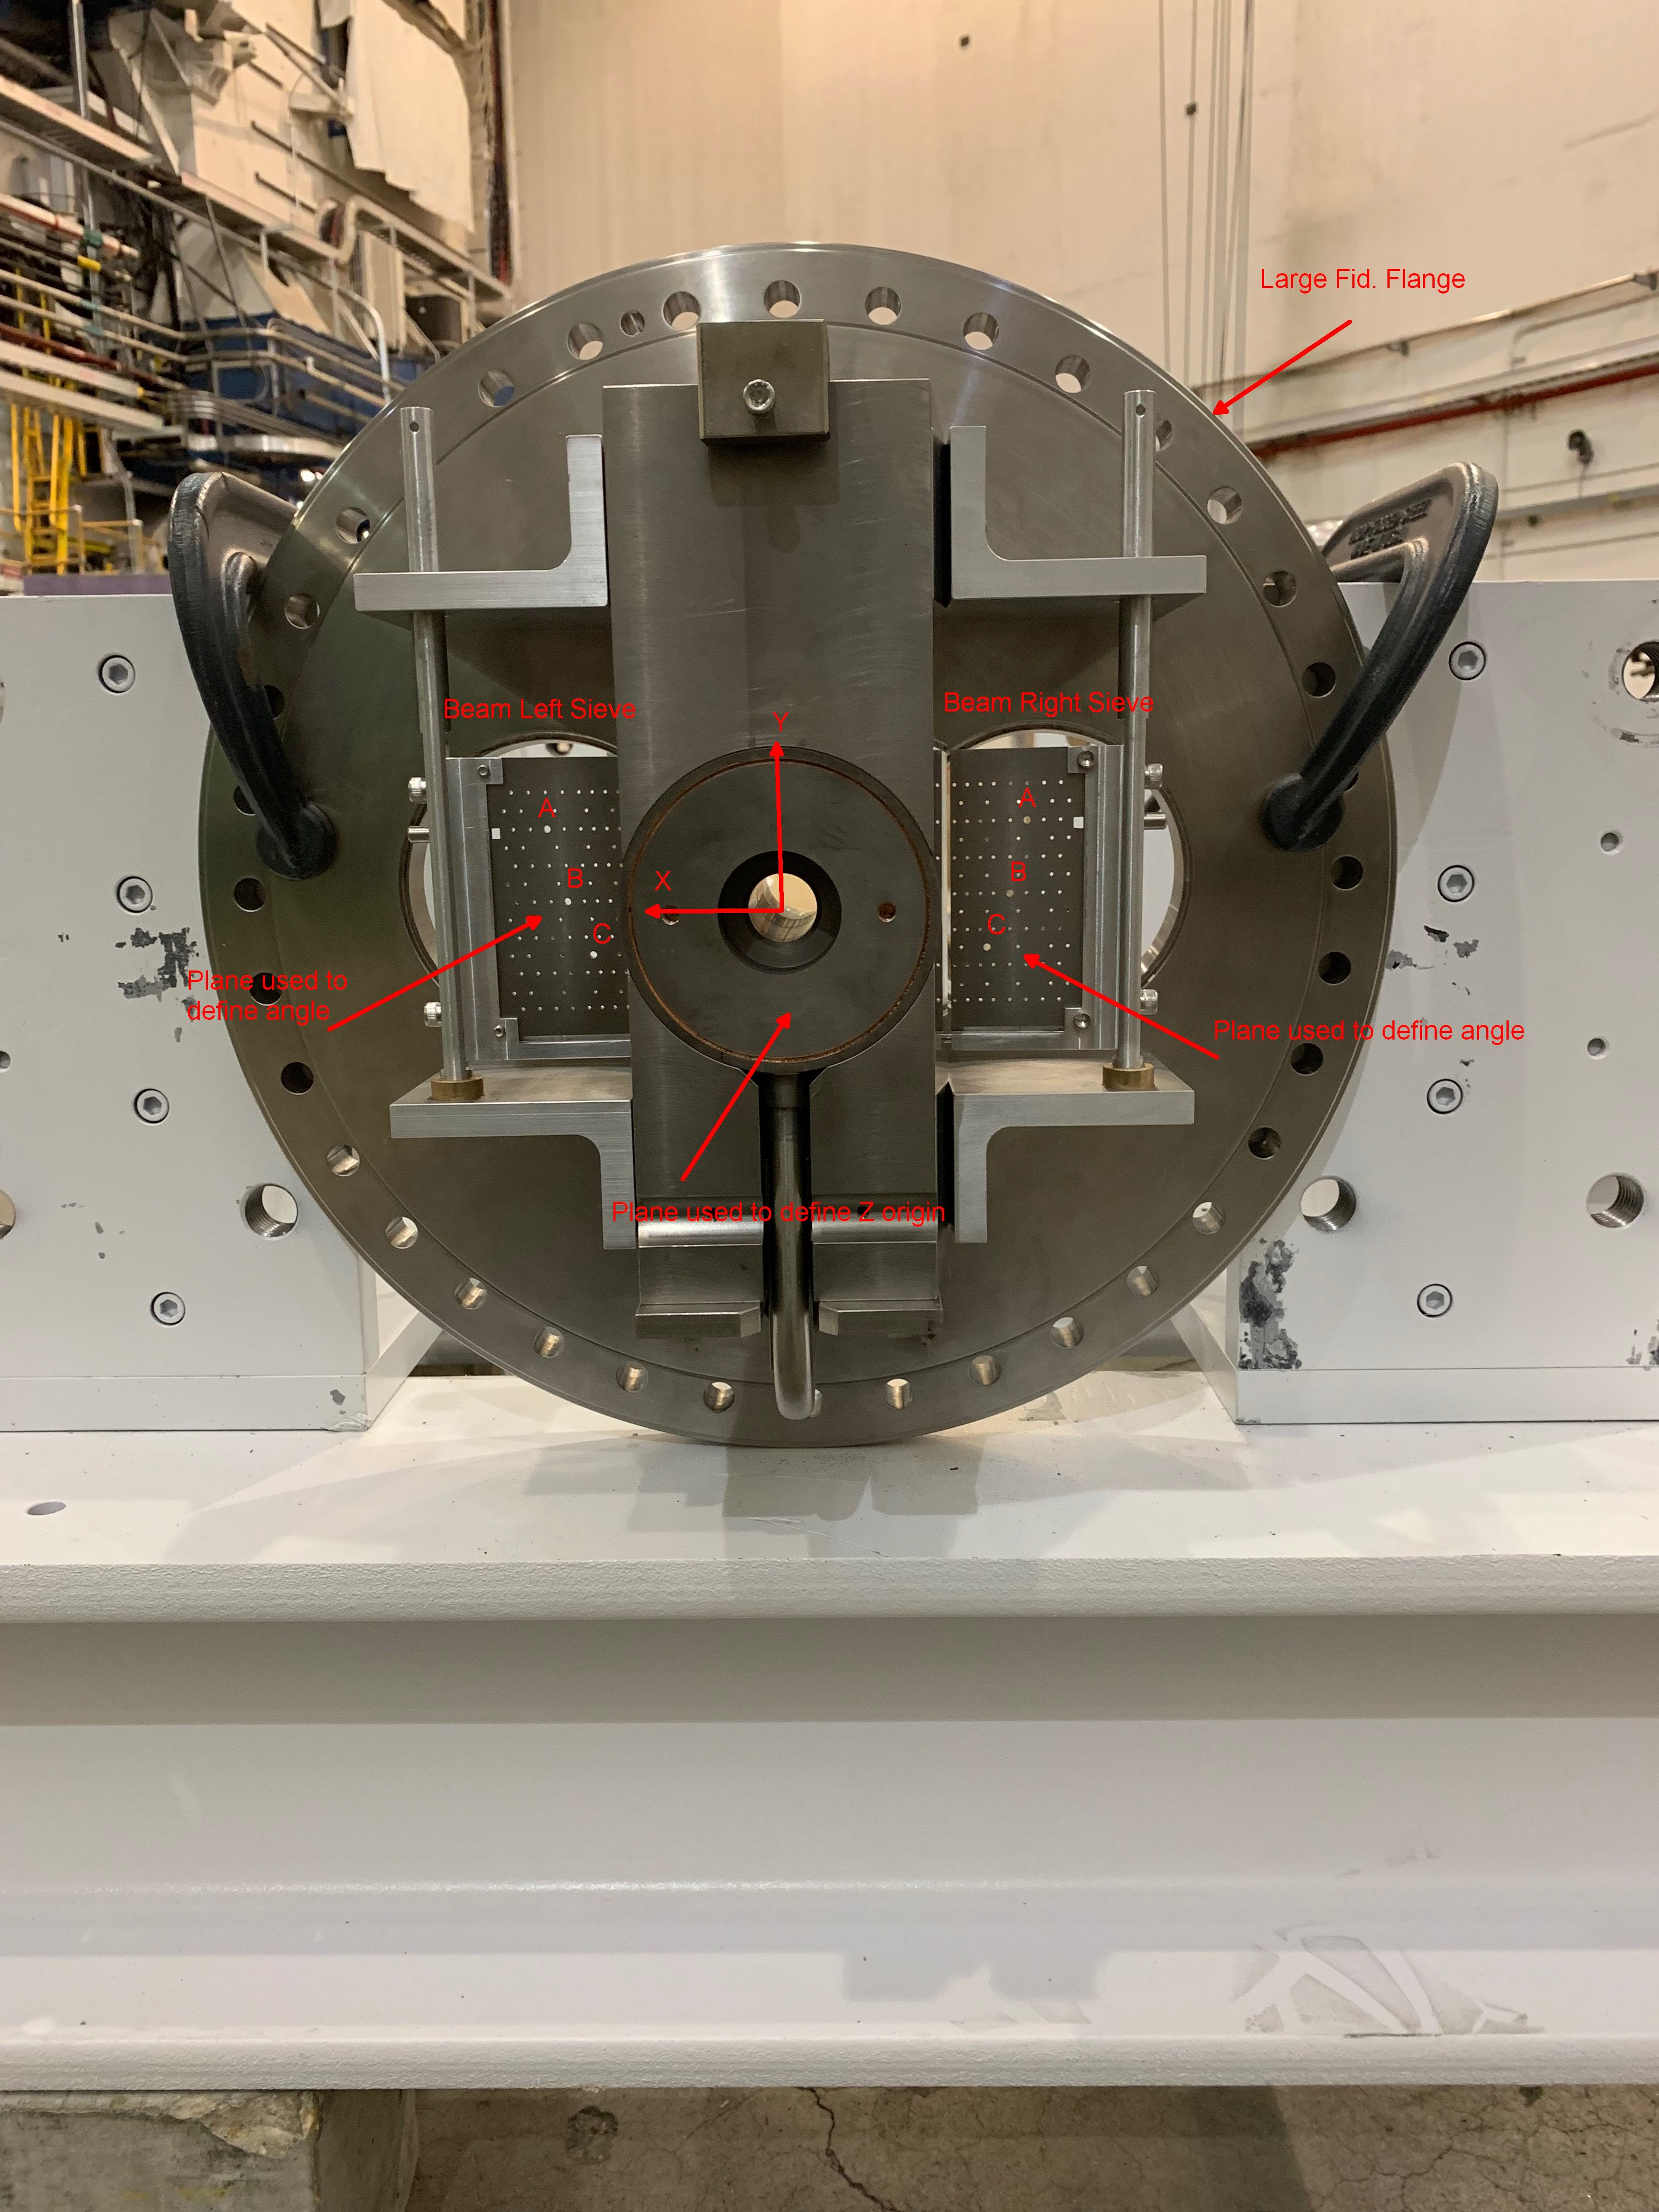
\includegraphics[width =\textwidth]{images/chap4/sieve_in_hrs.jpg}
    \caption{PRex-II/CRex Sieve slit in the High-resolution spectrometer}
    \label{fig:labeled_sieve_in_hrs}
\end{figure}


\begin{figure}
    \centering
    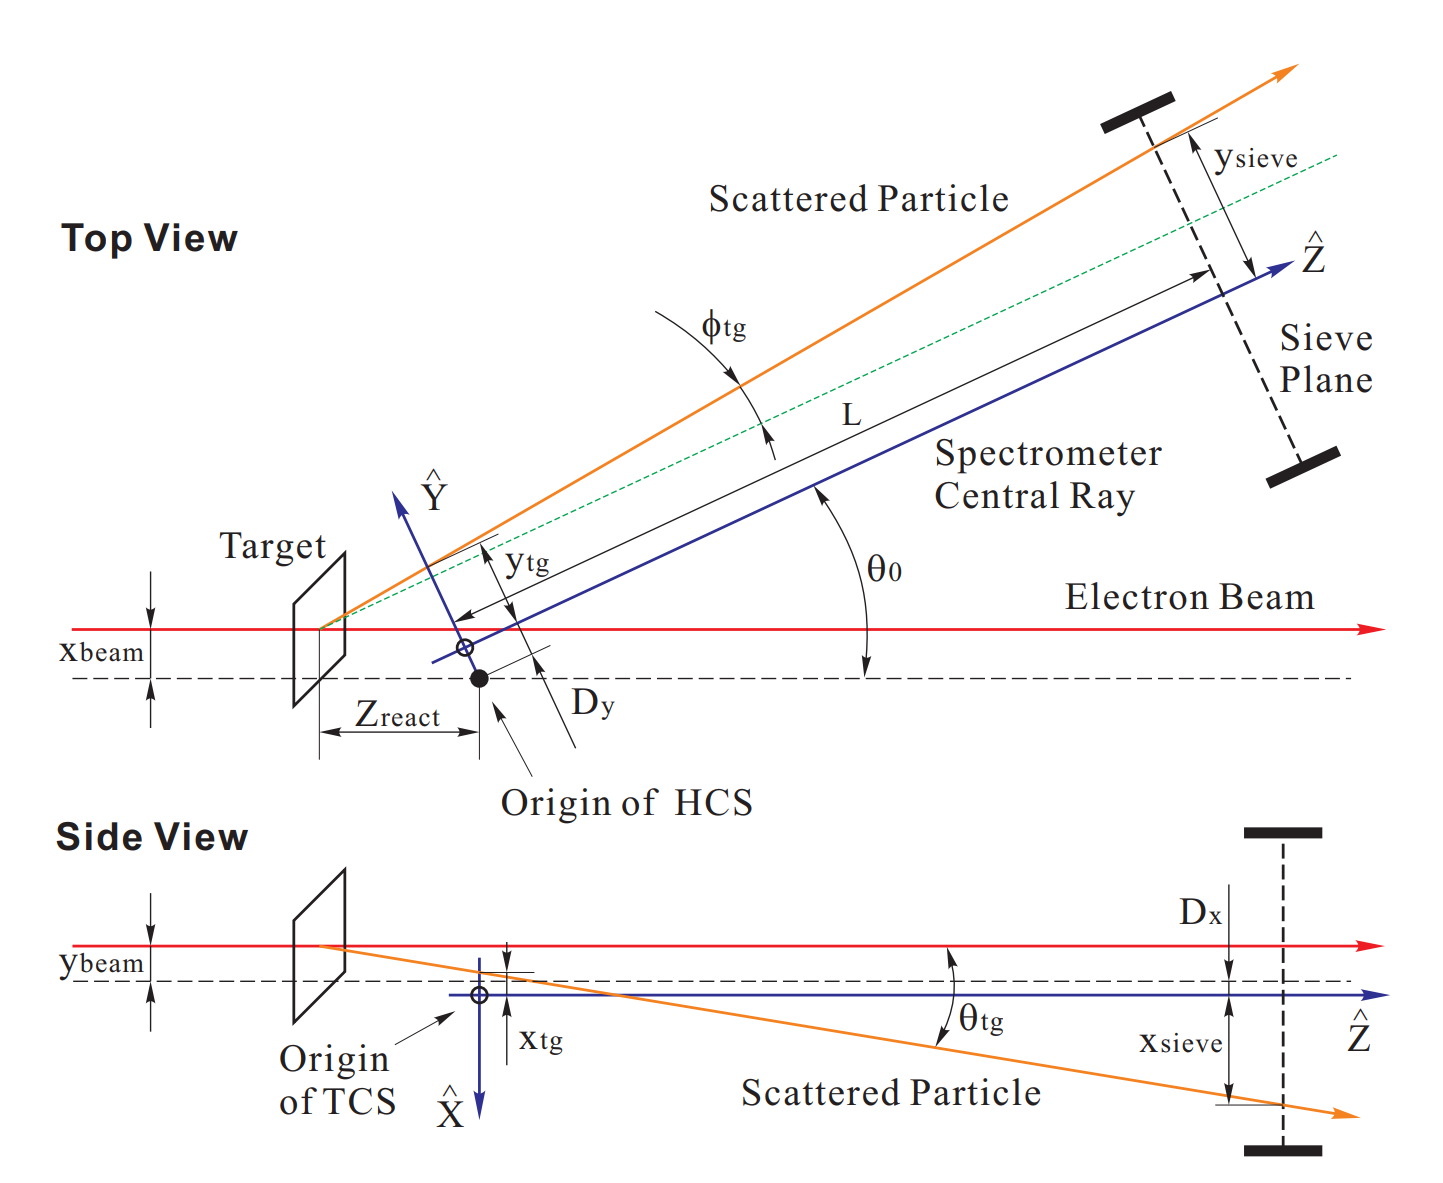
\includegraphics[width =\textwidth]{images/chap4/target_coordinate_system.png}
    \caption{Target Coordinate System}
    \label{fig:target_coordinate_system_plot}
\end{figure}

Figure \ref{fig:sieve_cnc_draw} displays the schematic of the sieve plate. The Hall A survey is conducted in the Hall A coordinate system and measured relative to the center of the sieve plate. In the target coordinate system, the origins of both the target and hall coordinate systems are assumed to be identical. However, in practice, the center of the target coordinate system deviates from that of the hall coordinate system. These deviations in the horizontal and vertical directions are denoted by $D_y$ and $D_x$, respectively. The ground truth result in the target coordinate system can be computed using the following equations:

\begin{equation}
\phi_{tg} = \frac{y_{sieve} + D_y - x_{beam}\cos{\theta_0} + z_{react}\sin{\theta_0}}{L - z_{react}\cos{\theta_0 - x_{beam}\sin{\theta_0}}}
\end{equation}

\begin{equation}
\theta_{tg} = \frac{x_{sieve} + D_x + y_{beam}}{L - z_{react}\cos{\theta_0} - x_{beam}\sin{\theta_0}}
\end{equation}

\begin{equation}
y_{tg} = y_{sieve} - L \phi_{tg}
\end{equation}

\begin{equation}
x_{tg} = x_{sieve} - L \theta_{tg}
\end{equation}

Where in the equation $\theta_0$ is the spectrometer central angle measured by the angle of the beam down direction and the central sieve hole. $L$ is the distance from the target location to the central sieve slit hole. Using these equations, the scattered angle and reaction point can be determined with the help of the beam variables measured in the hall coordinate system, as given by:

\begin{equation}
\theta_{scatter} = \arccos\left(\frac{\cos{\theta_0} - \phi_{tg}\sin{\theta_0}}{\sqrt{1 + \theta^2_{tg} + \phi^2_{tg}}}\right)
\end{equation}

\begin{equation}
z_{react} = \frac{-(z_{tg} + D_y) + x_{beam}(\cos{\theta_0} - \phi_{tg}\sin{\theta_0})}{\cos{(\theta_0\phi_{tg} + \sin{\theta_0})}}
\end{equation}

For the PRex-II experiment, only one target foil was employed. As a result, $z_{react}$ and $x_{react}$ are both 0. The constant spectrometer length $L$ and the central sieve angle in the Hall Coordinate System (HCS) are calculated using the survey results. For PRex-II experiment, the equations can be rewritten as:

\begin{equation}
    \theta_{tg} = \arctan{\frac{x_{sieve}}{L}}
\end{equation}

\begin{equation}
    \phi_{tg} = \arctan{\frac{y_{sieve} - x_{beam}\cos{\theta_0} + D}{L - x_{beam}\sin{\theta_0}}}
\end{equation}

\begin{equation}
    y_{tg} = y_{sieve} - L \frac{y_{sieve}-x_{sieve}\cos{\theta_0} + D}{L - x_{sieve}\sin{\theta_0}}
\end{equation}

After getting the ground truth values, with the help of the spectrometer tensor, we can project the measurement from the focal plane coordinate system to the target system, which is considered to be the predicted value in the optimization procedure. The loss function takes L2 loss, which is the square error between the predicted value and the ground truth. 


\subsubsection{Labeling the Ground Truth Dataset}

Before computing the ground truth values on the target using the previously discussed equations, it is crucial to know which sieve hole the event originates from. This information is necessary because the calculation involves determining parameters based on the geometric position of the sieve hole from which the particle comes. To obtain this data, an initial calibration tensor should be provided, and all events should be plotted on the target coordinate system. In this system, events are manually selected based on their patterns, and identical labels are assigned to all events within the same cluster.

The sample plot demonstrates the cut boundaries for the cluster on the target coordinate system, where the red circle represents the boundary. All events within this boundary are considered to have originated from the same sieve hole and, consequently, share similar properties such as scattered angle, $\theta_{tg}$, $\phi_{tg}$, four-momentum transfer, and so on.

Determining the sieve pattern can be challenging, and different individuals may have varying boundary criteria. To minimize errors caused by inconsistent criteria, a newly developed method was employed in practice. After identifying the rough center of a given cluster, the code places a large circle around the clicked center. Within this circle, event density contour lines are drawn, and the chosen contour line serves as the cut boundary for the event. This approach helps ensure more accurate and consistent boundary determination. The code for labeling the ground truth dataset can be found in this \href{https://github.com/Jiansiyu/GeneralScripts/blob/master/OptCut/CRexCut/cutPro.C}{GitHub repository}.


\subsection{Angular variable calibration}

The ground truth dataset is obtained from various beam positions and central momenta to cover a larger area of the vertical drift chamber. Figure \ref{fig:lhrs_tg_theta_phi_postopt} and \ref{fig:rhrs_tg_theta_phi_postopt} display the sieve patterns after the optics optimization. Each circle represents a cluster of events, while the green grid indicates the expected position for the sieve pattern.

Figures \ref{fig:lhrs_tg_theta_phi_residual} and \ref{fig:rhrs_tg_theta_phi_residual} show the residuals of the sieve events, grouped by events that pass through the same sieve hole. The green line represents the ideal case, which is the residual between the predicted and theoretical values. In practice, the residual cannot equal zero. The error bars represent the standard error of all events passing through the same sieve hole. The following table shows the optimization error for the PRex-II experiment (here takes the largest residual as the error).

\begin{figure}[h]
    \centering
    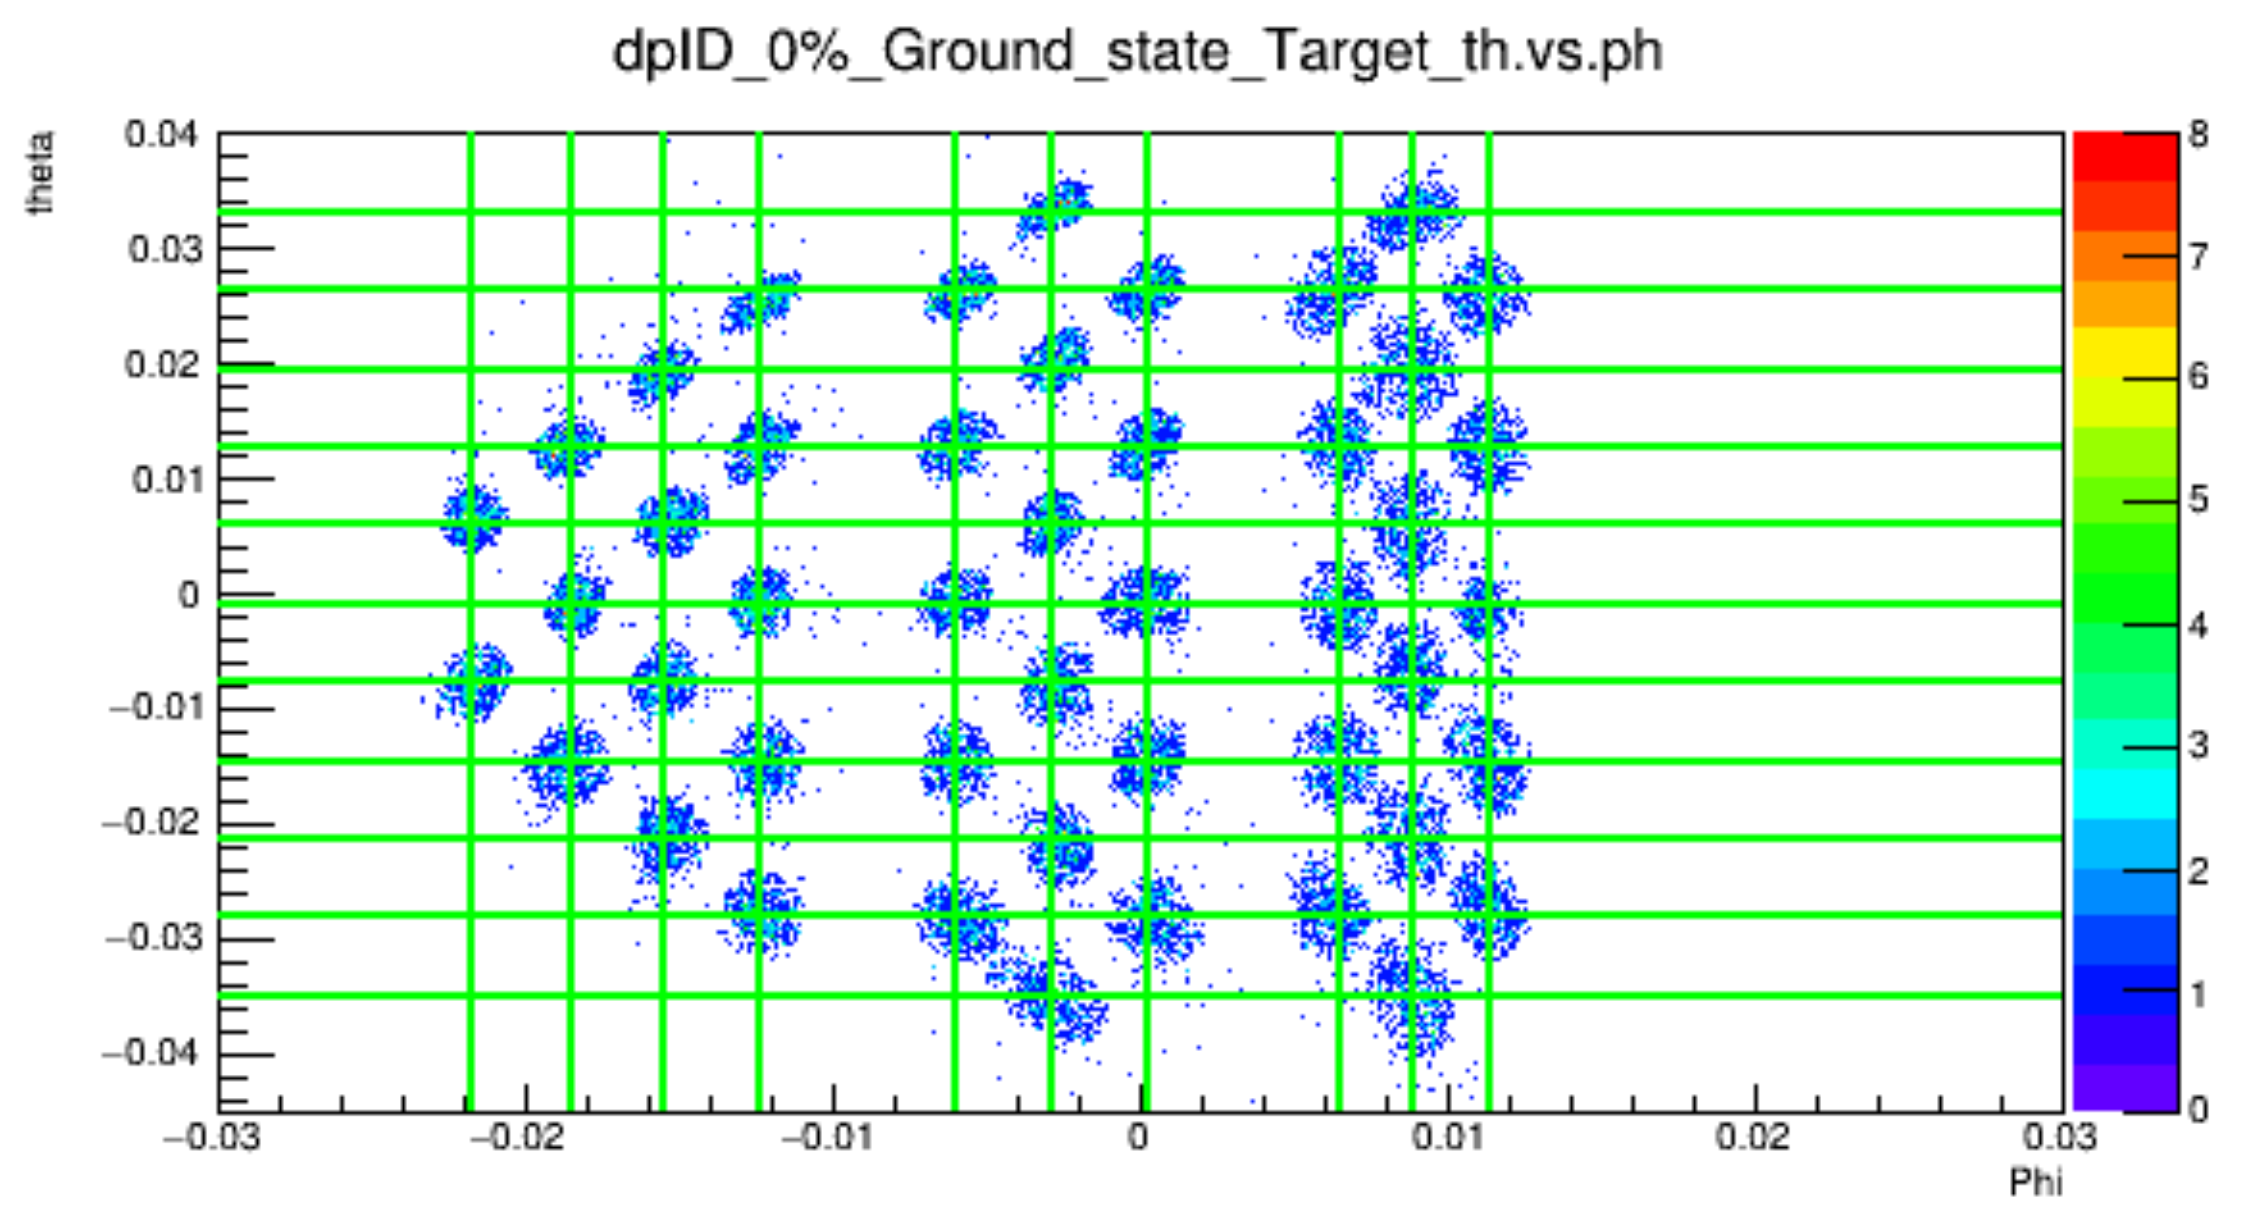
\includegraphics[width =\textwidth]{images/chap4/LHRS_tg_theta_phi_after_opt.png}
    \caption{LHRS Target $\theta_{tg}$ vs. $\phi_{tg}$ on target coordinate system}
    \label{fig:lhrs_tg_theta_phi_postopt}
\end{figure}

\begin{figure}[h]
    \centering
    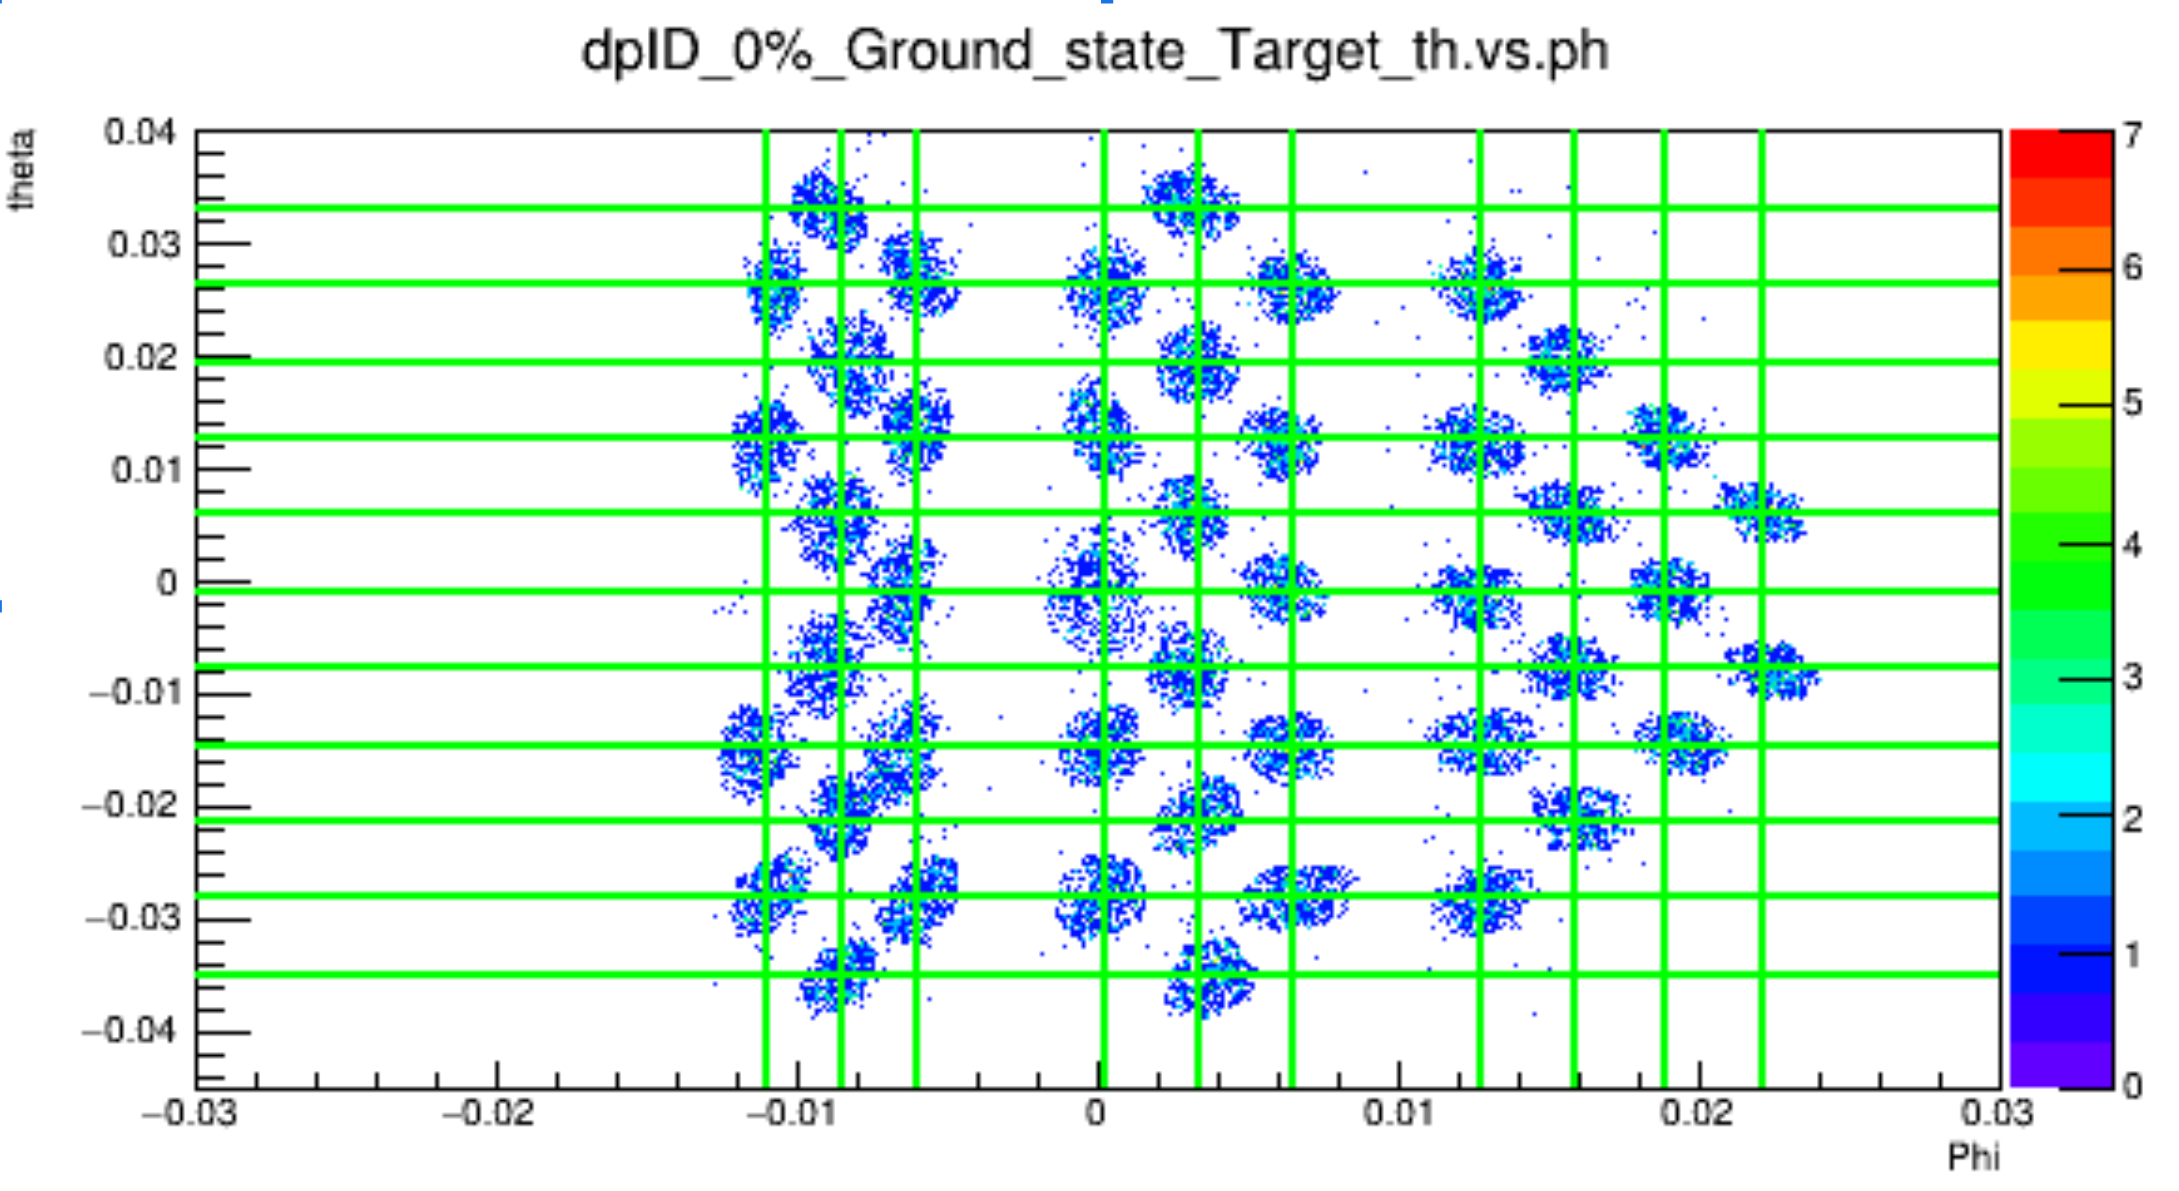
\includegraphics[width =\textwidth]{images/chap4/rhrs_tg_theta_phi_after_opt.png}
    \caption{RHRS Target $\theta_{tg}$ vs. $\phi_{tg}$ on target coordinate system}
    \label{fig:rhrs_tg_theta_phi_postopt}
\end{figure}

\begin{figure}[h]
    \centering
    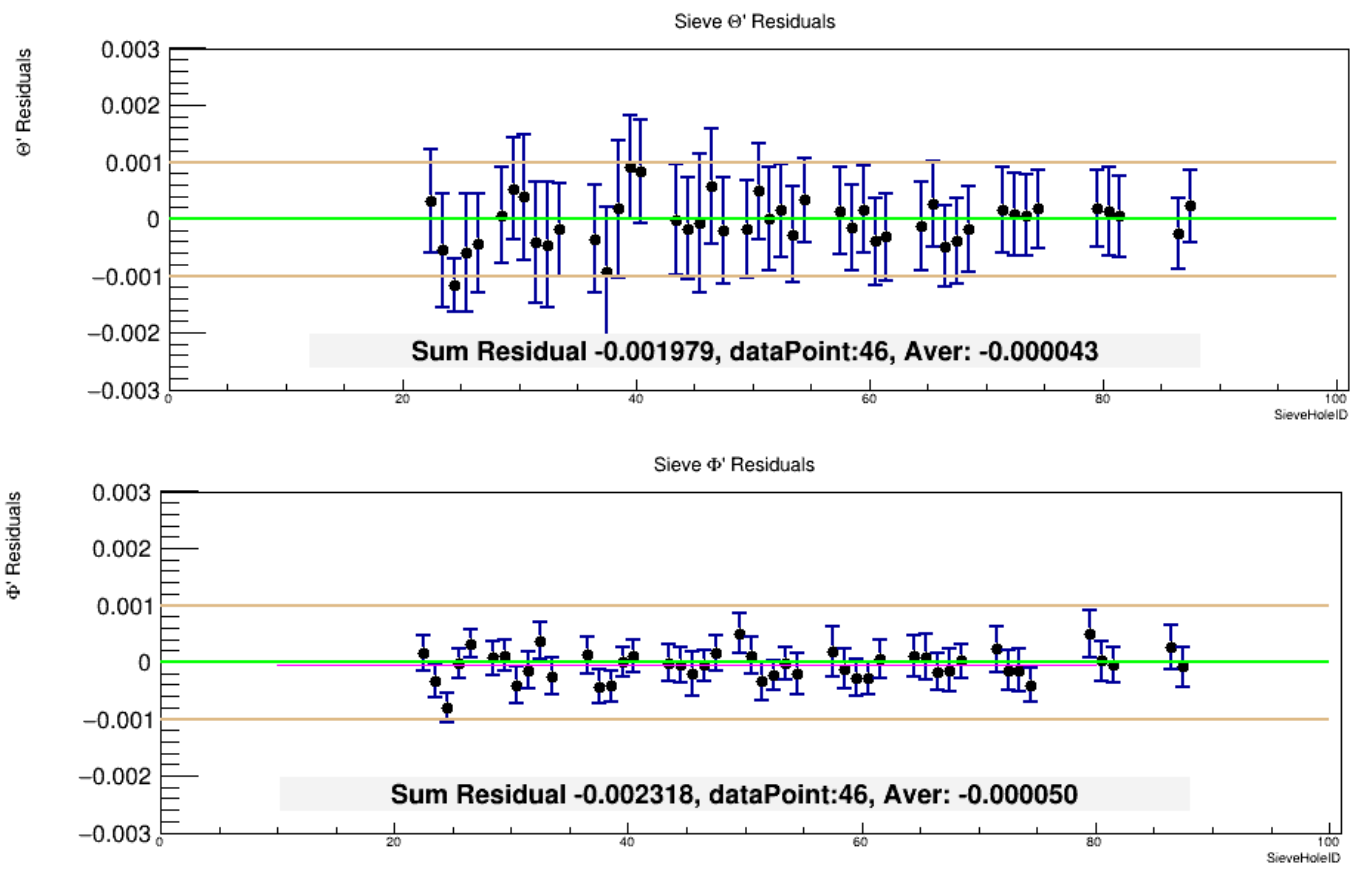
\includegraphics[width =\textwidth]{images/chap4/lhrs_tg_residual_plot.png}
    \caption{LHRS Target $\theta_{tg}$ and $\phi_{tg}$ Optimization Residual on Target Coordinate System}
    \label{fig:lhrs_tg_theta_phi_residual}
\end{figure}

\begin{figure}[h]
    \centering
    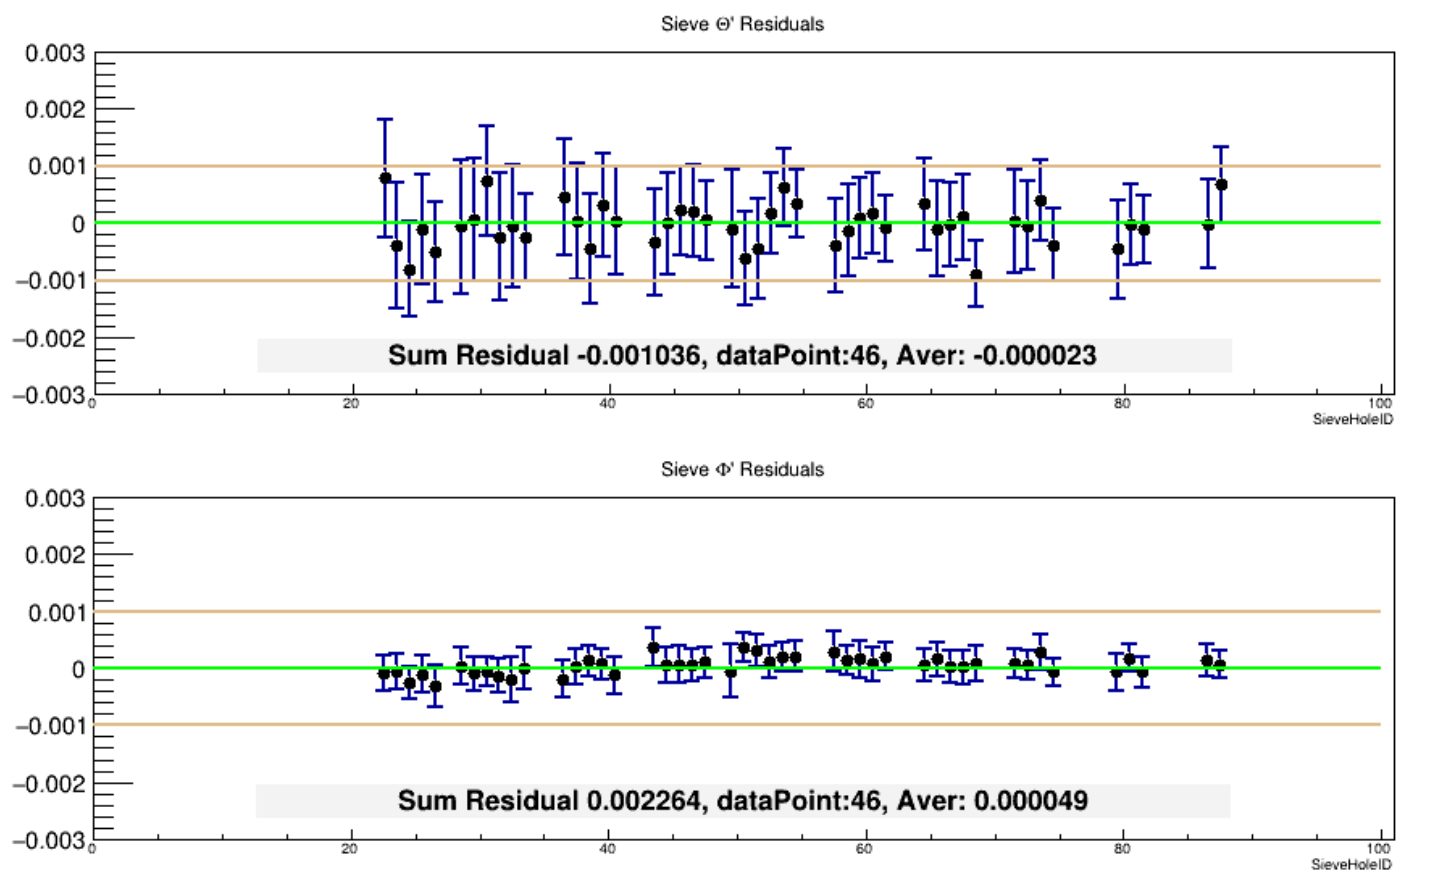
\includegraphics[width =\textwidth]{images/chap4/rhrs_residual_theta_phi.png}
    \caption{RHRS Target $\theta_{tg}$ and $\phi_{tg}$ Optimization Residual on Target Coordinate System}
    \label{fig:rhrs_tg_theta_phi_residual}
\end{figure}

\begin{center}
    \begin{tabular}{|c || c | c|}
        \hline
        \multicolumn{3}{|c|}{Angular Variable Calibration Accuracy} \\
        \hline
            HRS & $\theta$ & $\phi$ \\
        \hline
            RHRS & -1.57 mrad & 0.32 mrad \\
        \hline
            LHRS & 0.732 mrad & -0.492 mrad \\
            \hline
    \end{tabular}
\end{center}

\subsection{Momentum Calibration}
\subsubsection{Momentum Ground truth}

The scattering angle represents the angle between the direction of the scattered electrons and the direction of the electron beam. Standard survey procedures do not directly measure the scattering angle; instead, they measure the spectrometer central angle and the geometric positions of the sieve plate. The scattering angle can be calculated using the spectrometer central angle and the $\theta_{tg}$ and $\phi_{tg}$, which are determined based on the geometric position of the sieve hole relative to the central sieve hole. Given these parameters, the scattering angle can be calculated as:

\begin{equation} \label{eq:chapter4_scattered_angle_from_central_angle}
\theta = \frac{\cos{\theta_0} - \phi_{tg}\sin{\theta_0}}{\sqrt{1 + \theta^2_{tg} + \phi^2_{tg}}}
\end{equation}

With the scattering angle, the ground truth scattered electron momentum can be calculated as:

\begin{equation}
 p = \frac{E}{1 + \frac{2E}{M_c}(1 - \cos{\theta})}
\end{equation}


\subsubsection{Momentum Calibration result}
As stated in the equations, to simplify the complexity and facilitate model conversion, the momentum calibration is optimized using $\delta = \frac{p - p_0}{p_0}$. Similar to $\theta$ and $\phi$, the optimization needs to be performed separately for the LHRS and RHRS. The ground truth value incorporates the central sieve angle and the angle of the sieve hole in the target coordinate system within the sieve plate. The L2 loss function is employed, which calculates the sum of squared residuals between the ground truth $\delta p$ and the $\delta p$ computed using the projected momentum with the HRS tensor.

To cover a broader momentum range, data are taken with central momenta at $-1\%$, $0\%$, and $1\%$ of the standard central sieve momentum. Figures \ref{fig:lhrs_dp_residual} and \ref{fig:rhrs_dp_residual} display the residuals for LHRS and RHRS. Similar to the sieve $\theta$ and $\phi$ residual plots, data are grouped by the sieve hole. The beam energy of the accelerator is $952.9 MeV$.

The table below presents the error bars for the momentum optimization. The error is considered to be the largest residual difference compared to the theoretical value.

\begin{center}
    \begin{tabular}{|c || c |}
        \hline
        \multicolumn{2}{|c|}{Momentum Calibration Accuracy} \\
        \hline
            HRS & Momentum Error \\
        \hline
            RHRS & $\pm 0.5MeV$ \\
        \hline
            LHRS & $\pm 0.3MeV$ \\
        \hline
    \end{tabular}
\end{center}


\begin{figure}[h]
    \centering
    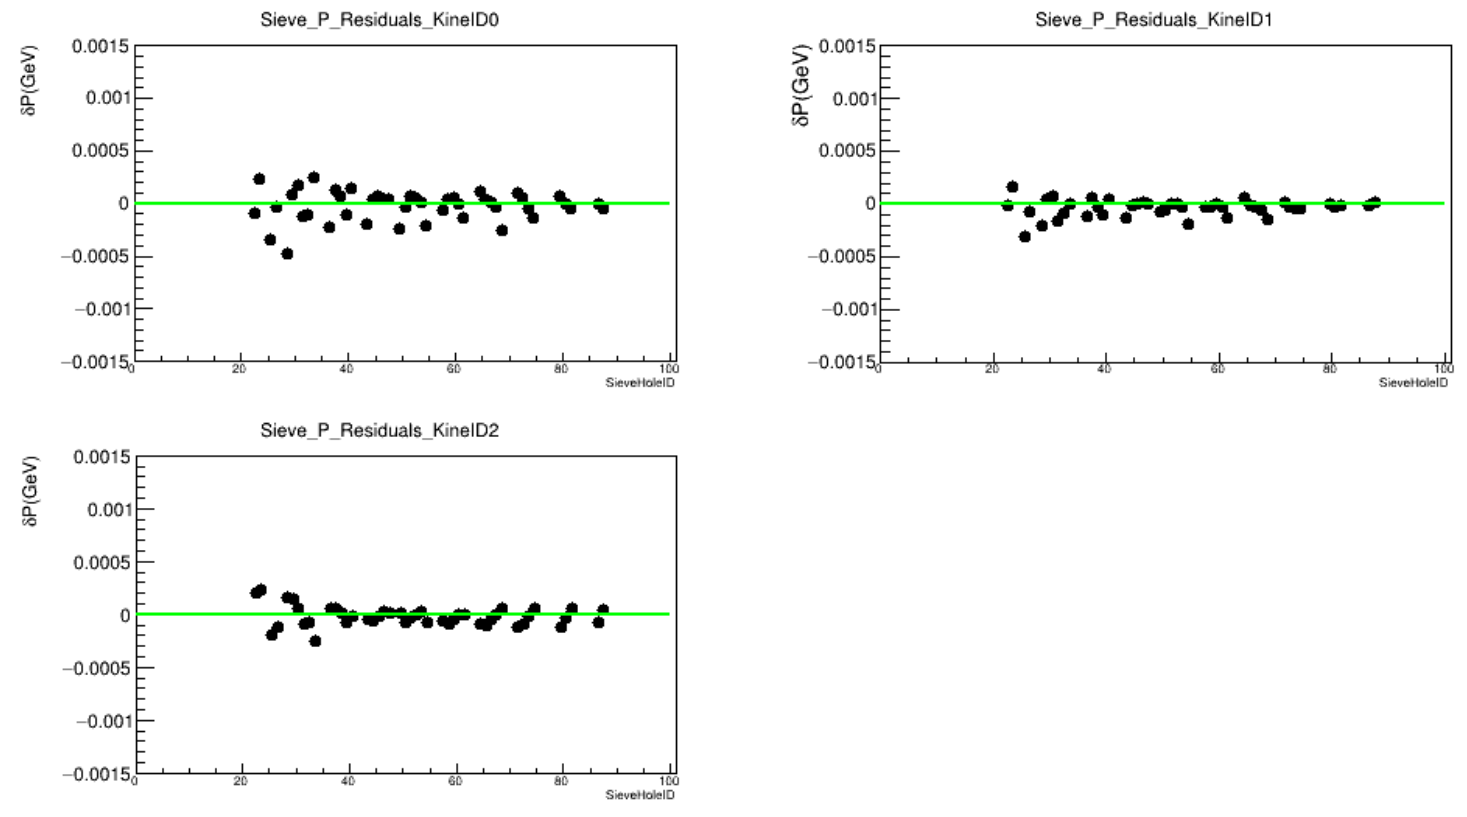
\includegraphics[width =\textwidth]{images/chap4/lhrs_dp_residual.png}
    \caption{Caption}
    \label{fig:lhrs_dp_residual}
\end{figure}


\begin{figure}[h]
    \centering
    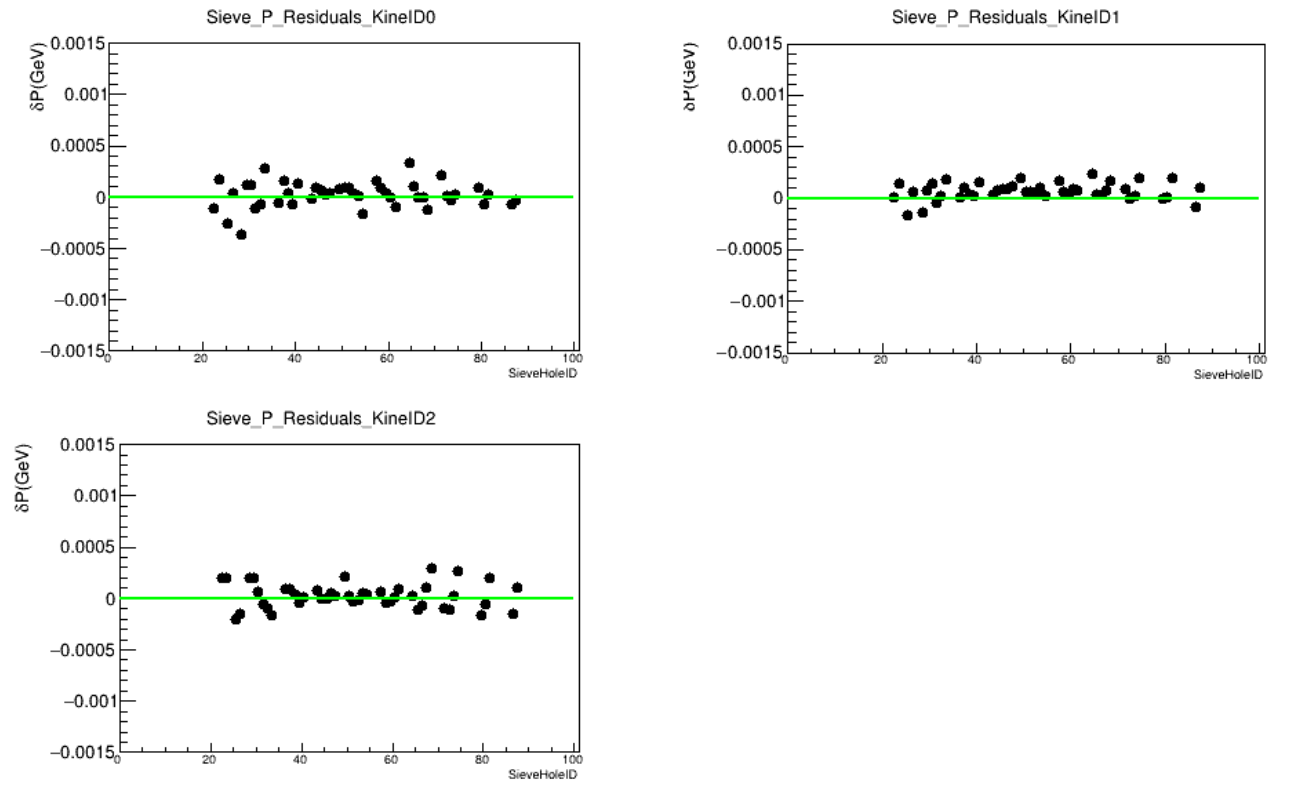
\includegraphics[width =\textwidth]{images/chap4/rhrs_dp_residual.png}
    \caption{Caption}
    \label{fig:rhrs_dp_residual}
\end{figure}

\section{Spectrometer central angle $\theta_0$ measurement }

The spectrometer central angle, $\theta_0$, is defined as the angle between the beam down direction and the central spectrometer axis. As shown in equation \ref{eq:chapter4_scattered_angle_from_central_angle}, the spectrometer's central angle serves as a fundamental input for calculating the particle scattered angle. The laser survey provides the spectrometer's central angle. $\theta_0$ can be measured using a survey that measures the angle between two imaginary lines: the first line runs along the ideal spectrometer axis, and the second line runs along the ideal electron beam direction.

However, multiple transformations are required to relate the ideal spectrometer angle to the actual spectrometer angle, which could increase the uncertainty of the $\theta_0$ measurement to as much as 0.06 or approximately $1\%$. This could, in turn, lead to a $2\%$ uncertainty in Q2 measurement in the case of the PREX experiment. In PRex Experiment, the measurement is through pointing measurement. This technique utilizes the concept of differential nuclear recoil for elastic electron scattering off target nuclei of different masses. Pointing measurements are generally more accurate than surveys, as they do not require multiple transformations like surveys. Furthermore, the accuracy of pointing measurements can be significantly improved by considering differential nuclear recoils off different target nuclei present in the same target, such as water (H2O). This method has the advantages of suppressing uncertainties from estimating energy losses occurring before and after scattering and eliminating the issue of potential beam position shifting during the run. The primary uncertainty that contributes to the pointing measurement uncertainty arises from the ability to measure the energy difference between two different peaks. In the case of PREX, the accuracy was at the level of ~30 keV. [change needed]

Consider an electron scattered on a target with mass $M$. The scattered electron momentum can be written as:

\begin{equation}
E' = \frac{E - E_{loss1}}{1 + \frac{2(E-E_{loss1})\sin^2{\frac{\theta}{2}}}{M}} - E_{loss2}
\end{equation}

In this equation, $E$ represents the initial energy of the electrons, $\theta$ is the scattered angle, $E_{loss1}$ is the energy loss occurring before scattering, and $E_{loss2}$ is the energy loss occurring after scattering.

The water target contains both $^{1}H$ and $^{16}O$, enabling the scattering of two targets with precisely the same beam energy, scattered angle, and energy loss. The energy loss is canceled out, thus increasing the measurement accuracy. The scattered electron energy difference between oxygen and hydrogen can be given by:

\begin{equation}
\Delta{E'} = E'_O - E'_H = E (\frac{1}{1 + \frac{2E\sin^2{\frac{\theta}{2}}}{M_O}} - \frac{1}{1 + \frac{2E\sin^2{\frac{\theta}{2}}}{M_H}}) + corrections
\end{equation}

In this equation, the corrections are negligible. Both the beam energy and the masses of oxygen and hydrogen are measured with high accuracy. With the scattered momentum reconstructed from the vertical drift chamber and the above equation, the scattered angle can be measured.

The CRex experiment uses the exact same spectrometer configuration, but with a beam energy of 2.18 GeV, yielding a much cleaner energy spectrum. In data analysis, CRex data is used instead of PREX data to achieve higher accuracy measurements.

The pointing measurement was conducted with a sieve in place, and events passing through the central sieve hole were used in the pointing calculation with the beam position along the center of the Hall A Coordinate System. This approach eliminates errors caused by HRS optics reconstruction errors. Figure \ref{fig:pointing_h2o_spectrum} displays an example of the waterfall target spectrum for CRex RHRS run 21737. The first peaks on the left and right represent the ground state energies of $^{1}H$ and $^{16}O$, respectively. The energy difference is $\Delta E = 16.126 \pm 0.024 MeV$. In order to obtain a highly accurate central angle, the pointing measurements were performed with different central momenta. The scattered electrons will end up in different VDC areas with different central momenta. Each central momentum run can provide independent energy differences between the hydrogen and oxygen spectra. Accurate optics reconstruction allows different central momenta to yield different energy differences between the hydrogen and oxygen targets while maintaining the same scattering angles. This helps verify the calibration accuracy.

To avoid drift during the experiment, pointing measurements were conducted three times: once at the beginning, once during the experiment, and a final verification pointing measurement after the experiment. The final pointing measurement is the average of these runs. A table listing all the runs used in the pointing measurement is provided.

During the pointing process, although the beam position is set to (0,0), it cannot perfectly reach $(0,0)$ due to control errors. To account for errors caused by beam position, the final angle is corrected by $\frac{X_{bpm}}{Z_0}$, where $Z_0$ represents the distance from the target center to the sieve slide along the spectrometer central ray (verification required), and $X_{bpm}$ is the beam position in the $X$ direction in the Hall A coordinate system.  

\begin{table}[!ht]
    \caption{LHRS Dec-16-2019 Pointing measurement}
    \centering
    \begin{tabular}{|l|l|l|l|l|l|}
    \hline
        ~ & LHRS & Initial\_L & bpmX & Correct Angle & Corrected HRS \\ \hline
       \multirow{5}{5em}{Dp $0\%$} &  2671 & 4.771 & 1.070 & -0.062 & 4.833 \\  
        ~ & 2672 & 4.831 & 0.083 & -0.005 & 4.836 \\ 
        ~ & 2673 & 4.725 & 2.011 & -0.116 & 4.841 \\ 
        ~ & 2674 & 4.763 & 1.081 & -0.062 & 4.825 \\  
        ~ & 2675 & 4.787 & 1.008 & -0.058 & 4.845 \\ \hline
        \multirow{3}{5em}{ Dp $+1\%$} & 2709 & 4.749 & 0.936 & -0.054 & 4.803 \\ 
        ~ & 2710 & 4.806 & 0.094 & -0.005 & 4.811 \\  
        ~ & 2711 & 4.691 & 2.049 & -0.118 & 4.809 \\ \hline
        \multirow{5}{5em}{ Dp $-1\%$} & 2723 & 4.755 & 0.950 & -0.055 & 4.810 \\   
        ~ & 2724 & 4.808 & -0.029 & 0.002 & 4.806 \\  
        ~ & 2725 & 4.702 & 2.055 & -0.119 & 4.821 \\ 
        ~ & 2726 & 4.756 & 1.093 & -0.063 & 4.819 \\  
        ~ & 2727 & 4.771 & 1.017 & -0.059 & 4.830 \\ \hline
    \end{tabular}
    \label{table:crex_1_pointing_lhrs}
\end{table}


\begin{table}[!ht]
    \caption{RHRS Dec-16-2019 Pointing measurement}
    \centering

    \begin{tabular}{|l|l|l|l|l|l|}
    \hline
        ~ & RHRS & Initial\_R & bpmX & Correct Angle & Corrected HRS \\ \hline
        \multirow{5}{5em}{Dp $0\%$} & 21736 & 4.771 & 1.070 & 0.062 & 4.709 \\
        ~ & 21737 & 4.722 & 0.083 & 0.005 & 4.717 \\
        ~ & 21738 & 4.827 & 2.011 & 0.116 & 4.711 \\
        ~ & 21739 & 4.78 & 1.081 & 0.062 & 4.718 \\
        ~ & 21740 & 4.78 & 1.008 & 0.058 & 4.722 \\ \hline
        \multirow{3}{5em}{ Dp $+1\%$} & 21774 & 4.749 & 0.936 & 0.054 & 4.695 \\
        ~ & 21775 & 4.706 & 0.094 & 0.005 & 4.701 \\
        ~ & 21776 & 4.813 & 2.049 & 0.118 & 4.695 \\ \hline
        \multirow{5}{5em}{ Dp $-1\%$} & 21786 & 4.757 & 0.950 & 0.055 & 4.702 \\ 
        ~ & 21787 & 4.692 & -0.029 & -0.002 & 4.694 \\ 
        ~ & 21788 & 4.806 & 2.055 & 0.119 & 4.687 \\
        ~ & 21789 & 4.752 & 1.093 & 0.063 & 4.689 \\ 
        ~ & 21790 & 4.75 & 1.017 & 0.059 & 4.691 \\ \hline
    \end{tabular}
    \label{table:crex_1_pointing_lhrs}
\end{table}


\begin{table}[!ht]
    \caption{LHRS Aug-9-2020 Pointing measurement}
    \centering
    \begin{tabular}{|l|l|l|l|l|l|}
    \hline
        ~ & LHRS & Initial\_L & bpmX & corrected\_A & Corrected HRS \\ \hline
        \multirow{5}{5em}{Dp $0\%$} & 3108 & 4.716 & 1.981 & -0.1143 & 4.8303 \\  
        ~ & 3109 & 4.832 & 0.045 & -0.0026 & 4.8346 \\ 
        ~ & 3110 & 4.832 & 0.006 & -0.0003 & 4.8323 \\  
        ~ & 3111 & 4.713 & 1.896 & -0.1094 & 4.8224 \\  
        ~ & 3112 & 4.785 & 0.963 & -0.0555 & 4.8405 \\  \hline
        \multirow{2}{5em}{Dp $-1\%$} & 3113 & 4.758 & 0.980 & -0.0565 & 4.8145 \\ 
        ~ & 3114 & 4.754 & 0.989 & -0.0571 & 4.8111 \\ \hline
    \end{tabular}
    \label{table:crex_2_pointing_lhrs}
\end{table}

\begin{table}[!ht]
    \caption{RHRS Aug-9-2020 Pointing measurement}
    \centering
    \begin{tabular}{|l|l|l|l|l|l|}
    \hline
        ~ & RHRS & Initial\_R & bpmX & Correct Angle & Corrected HRS \\ \hline
        \multirow{5}{5em}{Dp $0\%$} & 22114 & 4.842 & 1.981 & 0.114 & 4.728 \\ 
        ~ & 22115 & 4.734 & 0.045 & 0.003 & 4.731 \\  
        ~ & 22116 & 4.743 & 0.006 & 0.000 & 4.743 \\  
        ~ & 22117 & 4.853 & 1.896 & 0.109 & 4.744 \\  
        ~ & 22118 & 4.788 & 0.963 & 0.056 & 4.732 \\ \hline
        \multirow{2}{5em}{Dp $-1\%$} & 22119 & 4.769 & 0.980 & 0.057 & 4.712 \\ 
        ~ & 22120 & 4.767 & 0.989 & 0.057 & 4.710 \\ \hline
    \end{tabular}
    \label{table:crex_2_pointing_rhrs}
\end{table}

\begin{table}[!ht]
    \caption{LHRS Sep-13-2020 Pointing measurement}
    \centering
    \begin{tabular}{|l|l|l|l|l|l|}
    \hline
        ~ & LHRS & Initial\_L & bpmX & corrected\_A & Corrected HRS \\ \hline
        \multirow{5}{5em}{Dp $0\%$} & 3278 & 4.773 & 0.985 & -0.057 & 4.830 \\  
        ~ & 3279 & 4.83 & 0.069 & -0.004 & 4.834 \\  
        ~ & 3284 & 4.721 & 2.007 & -0.116 & 4.837 \\  
        ~ & 3286 & 4.771 & 1.057 & -0.061 & 4.832 \\ 
        ~ & 3291 & 4.776 & 1.006 & -0.058 & 4.834 \\ \hline
        \multirow{2}{5em}{Dp $+1\%$}  & 3292 & 4.8 & 1.035 & -0.060 & 4.860 \\  
        ~ & 3299 & 4.802 & 1.049 & -0.060 & 4.862 \\ \hline
        \multirow{1}{5em}{Dp $-1.7\%$} & 3302 & 4.738 & 1.052 & -0.061 & 4.799 \\ \hline
    \end{tabular}
    \label{table:crex_3_pointing_lhrs}
\end{table}


\begin{table}[!ht]
    \caption{RHRS Sep-13-2020 Pointing measurement}
    \centering
    \begin{tabular}{|l|l|l|l|l|l|}
    \hline
        ~ & RHRS & Initial\_R & bpmX & Correct Angle & Corrected HRS \\ \hline
        \multirow{5}{5em}{Dp $0\%$} & 22234 & 4.789 & 0.985 & 0.057 & 4.732 \\ 
        ~ & 22235 & 4.741 & 0.069 & 0.004 & 4.737 \\ 
        ~ & 22240 & 4.849 & 2.007 & 0.116 & 4.733 \\ 
        ~ & 22242 & 4.812 & 1.057 & 0.061 & 4.751 \\  
        ~ & 22247 & 4.793 & 1.006 & 0.058 & 4.735 \\ \hline
        \multirow{2}{5em}{Dp $+1\%$} & 22248 & 4.791 & 1.035 & 0.060 & 4.731 \\ 
        ~ & 22255 & 4.786 & 1.049 & 0.060 & 4.726 \\ \hline
        \multirow{1}{5em}{Dp $-1.7\%$} & 22256 & 4.743 & 1.052 & 0.061 & 4.682 \\ \hline
    \end{tabular}
    \label{table:crex_3_pointing_rhrs}
\end{table}

\begin{figure}[h]
    \centering
    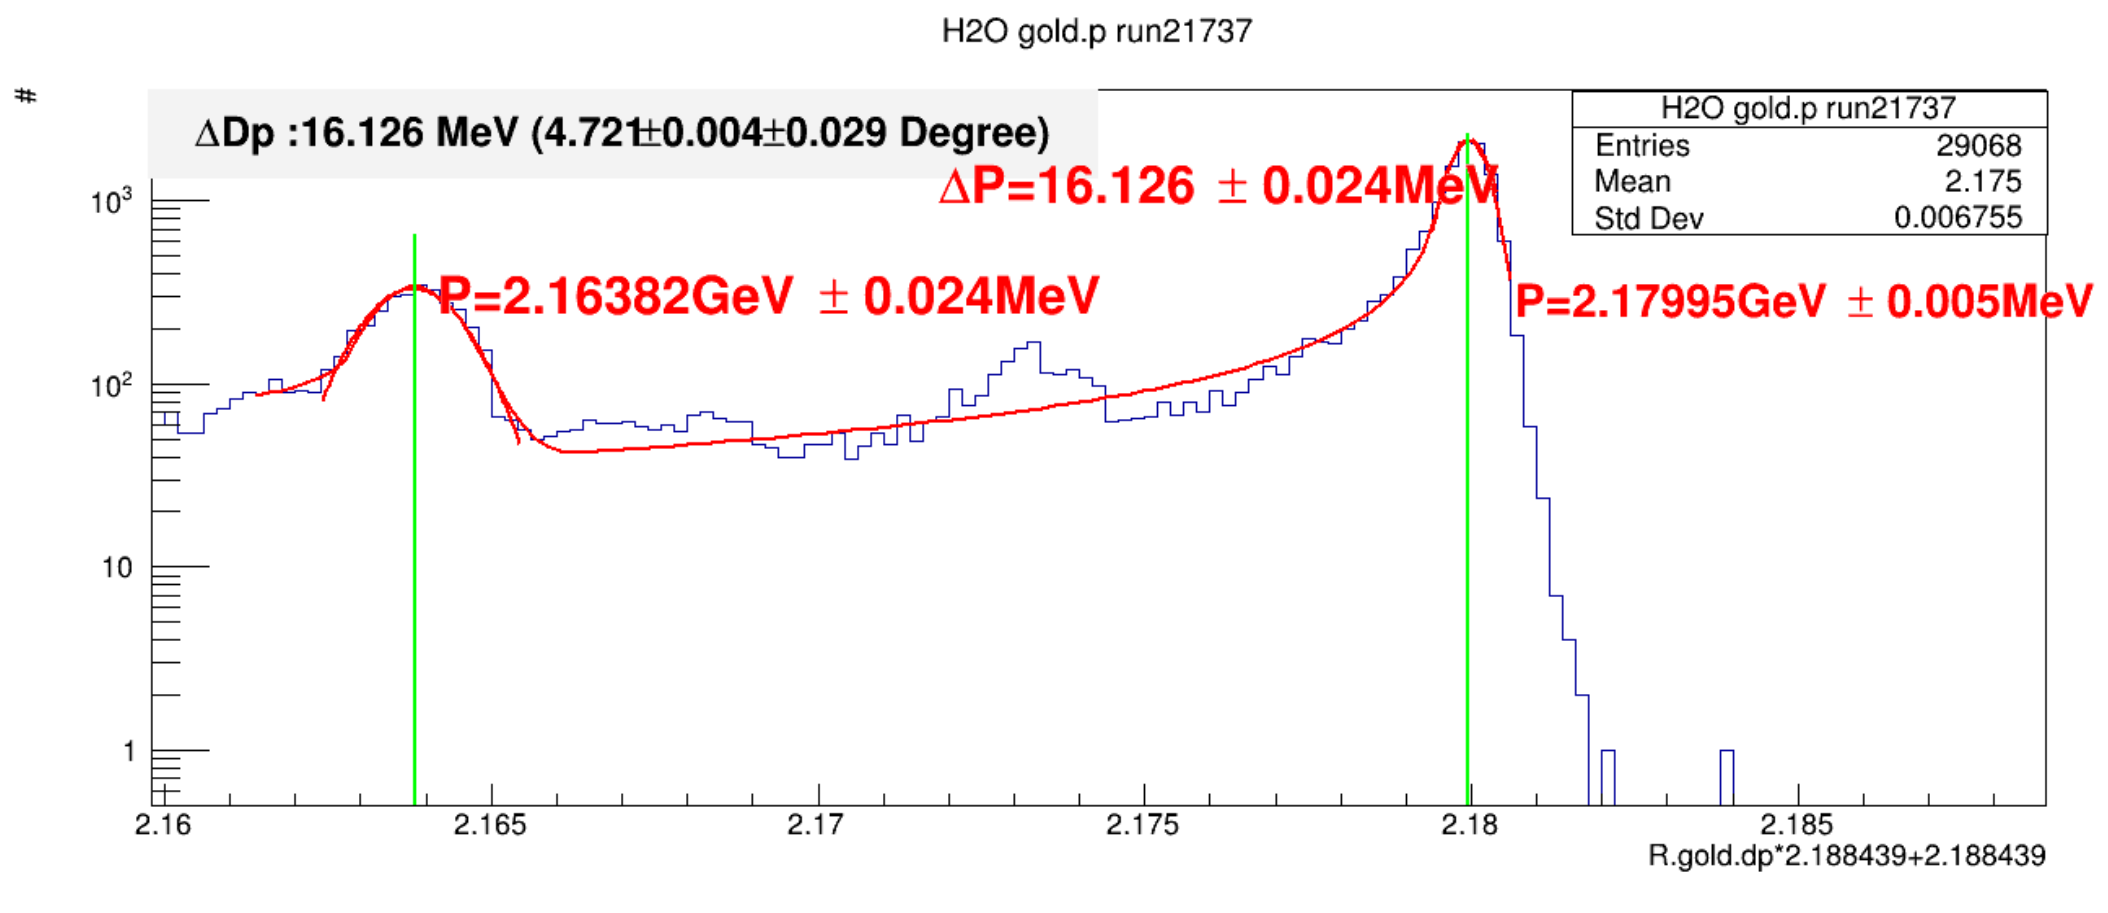
\includegraphics[width =\textwidth]{images/chap4/pointing_h20_spectrum.png}
    \caption{Caption}
    \label{fig:pointing_h2o_spectrum}
\end{figure}


\begin{figure}[h]
    \centering
    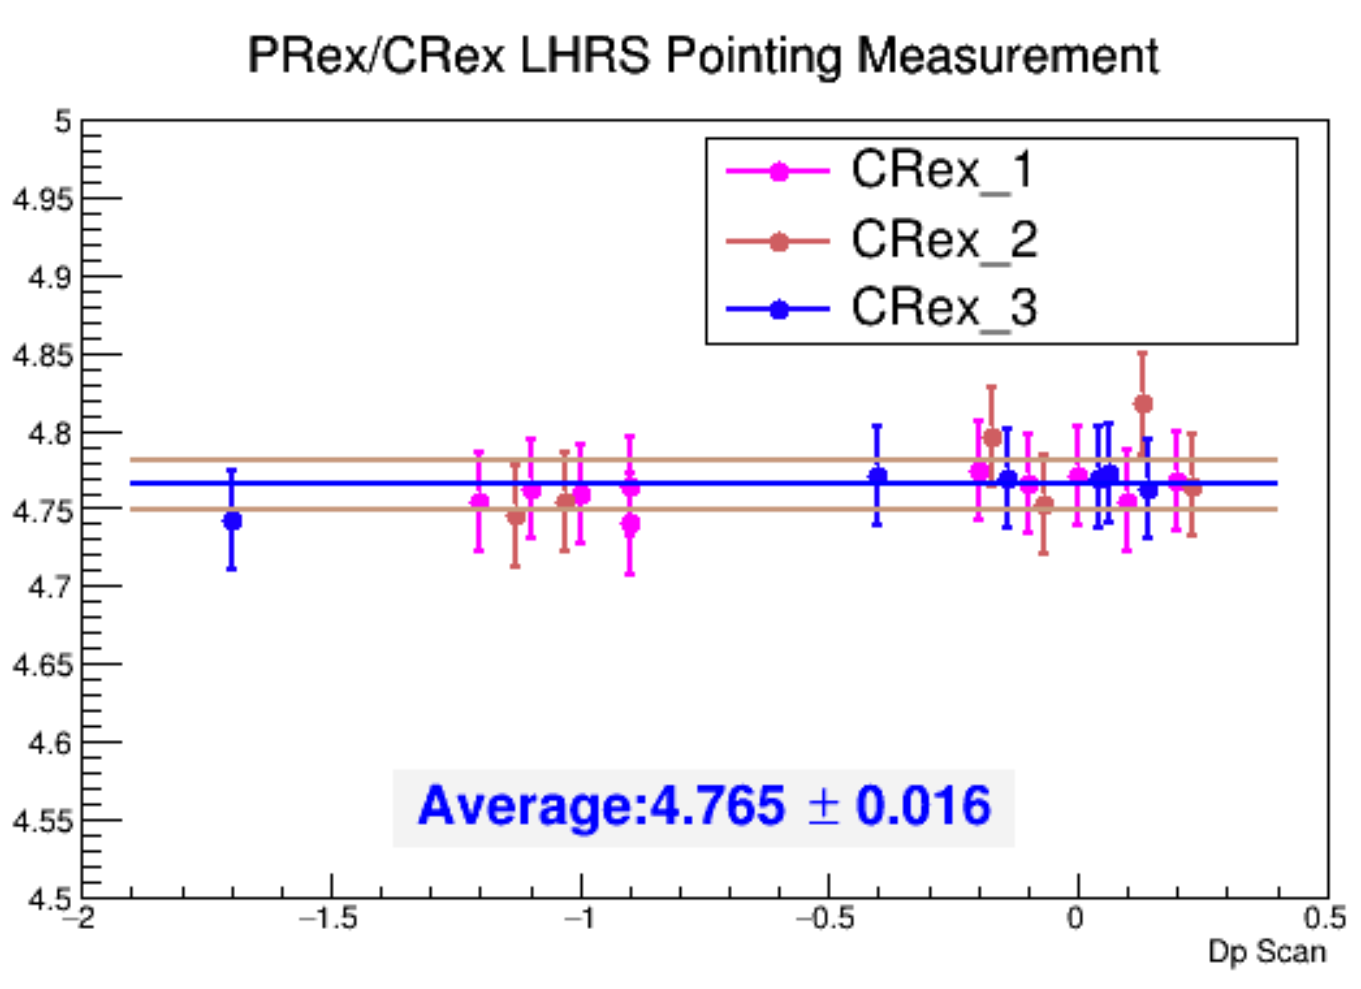
\includegraphics[width =\textwidth]{images/chap4/lhrs_pointing_summary.png}
    \caption{Caption}
    \label{fig:my_label}
\end{figure}

\begin{figure}[h]
    \centering
    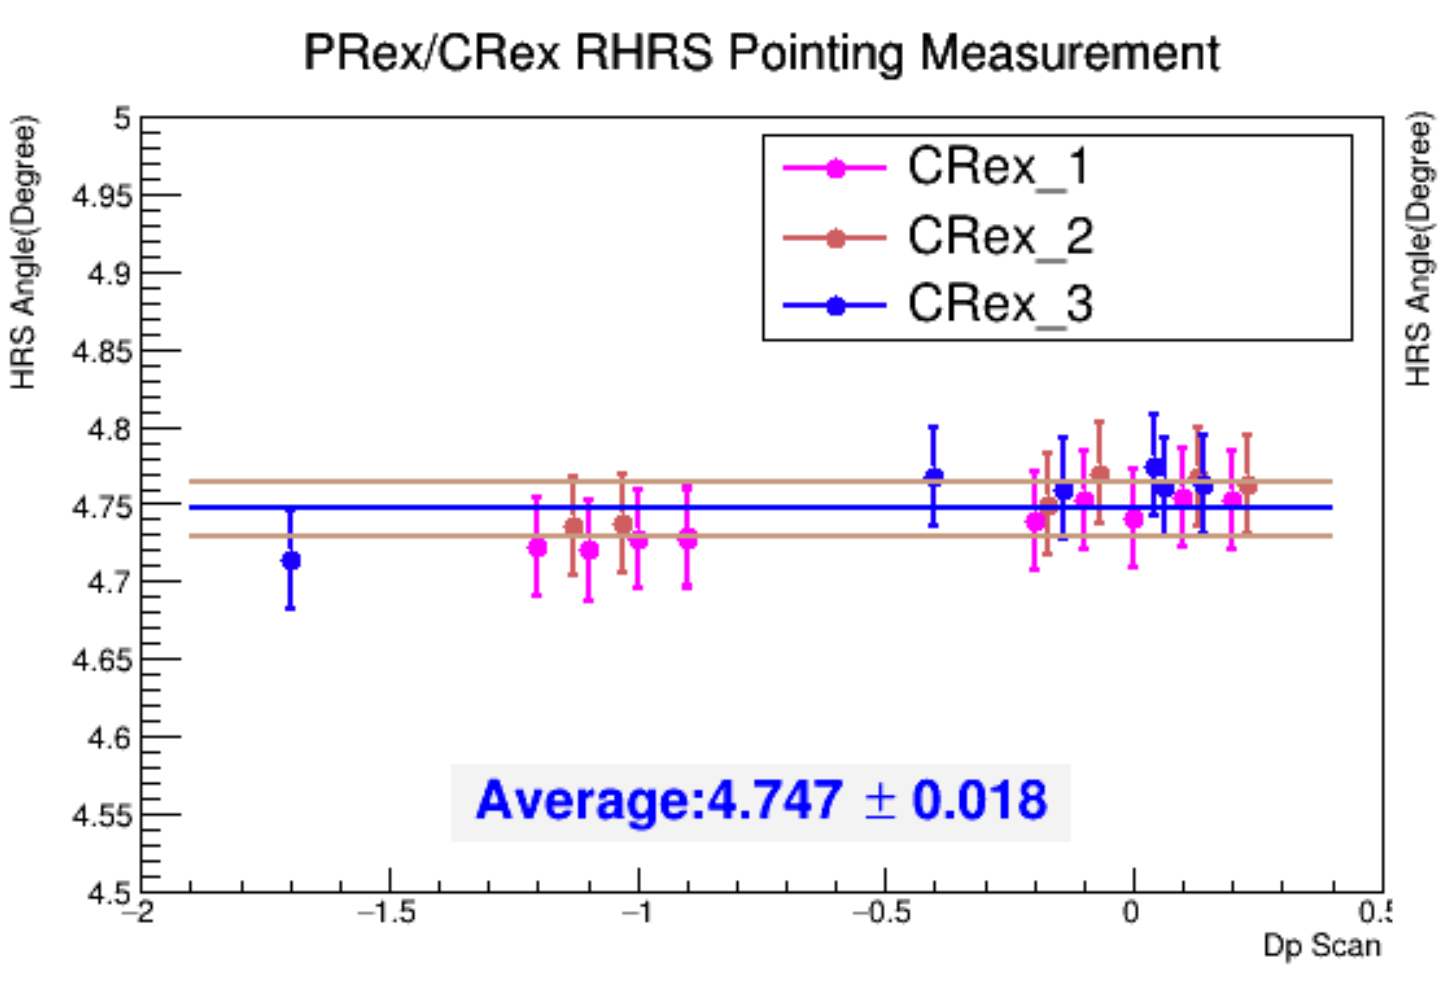
\includegraphics[width =\textwidth]{images/chap4/rhrs_pointing_summary.png}
    \caption{Caption}
    \label{fig:my_label}
\end{figure}

\href{https://docs.google.com/spreadsheets/d/12B7BL0aG4ZT-L9QYeQnX1PDxArS75PFv40Hdc3eRv4k/edit?usp=sharing}{data source, need to add that information}

\href{https://github.com/Jiansiyu/GeneralScripts/blob/master/PointingCheck/crex_pointing.csv}{Pointing measurement final result csv}


\section{$Q^2$ measurement}



% \subsubsection{beam position correction}

% \subsection{CRex experiment calibration}
% \subsection{a second thought on the optics optimization}


% Move to a separate chapter describing the apparatus and experiment details

% \begin{itemize}
%     \item Overview of the HRS structure
%     \item septum magnet 
%     \item Vertical drift chamber 
%     \item GEM detector
%     \item supporting equipment used for optimization only sieve slide

%     \item coordination system of the Jefferson Lab Hall A
%     \item coordination system of the HRS
% \end{itemize}


% \subsection{HRS model}

% \begin{itemize}
%     \item mathematical model of the HRS
%     \item constant parameter optimization
%     \item Vertical Drift Chamber time optimization
%     \item carbon calibration(dashed lines in the VDC spectrometer)
%     \item math why higher order contribute, a discussion notes
%     \item feature selection techniques
%     \item linear regression
%     \item result validation
%     \item result and discussion
% \end{itemize}
% \subsubsection{supervised linear regression}
% \subsubsection{feature selection technics}
% \subsubsection{mathematics about the linear regression, LASSO and ridge regression}

% \subsubsection{Linear Regression and mathematics approximation}




% \subsection{}section{feature selection}

% \subsubsection{general consideration in regression}

% \subsubsection{features in regression}

% \subsubsection{LASSO feature reduction regression}

% \subsubsection{ridge feature reduction regression}

% \subsection{autoML and more}

% \section{Momentum optimization}

% \section{Regression Result validation}

% \subsection{carbon result check}

% \subsubsection{first, second, third momentum check}

% \section{momentum reconstruction}

% \section{scattered angle reconstruction and correction}

% \section{a second thought/attempt on the regression}

% \subsection{another more complicated model}